\documentclass[MTech]{iitmdiss}

\usepackage{times}
\usepackage{epsf}
\usepackage{threeparttable}
\usepackage{setspace}
\usepackage{amsmath}
\usepackage{amsthm}
\usepackage{txfonts,pxfonts,amsfonts}
\usepackage{epsfig}
\usepackage{caption}
\usepackage{subfig}
\usepackage[dvips]{graphicx}
\usepackage[square,numbers,sort]{natbib}
\usepackage[square]{natbib}
\usepackage[hypertex]{hyperref} % hyperlinks for references.
%\usepackage{algorithmic}
%\usepackage{algorithm}
\usepackage{listings}
%\include{commands}

%\usepackage[pdftex]{graphicx}
% Strut macros for skipping spaces above and below text in tables. 
\def\abovestrut#1{\rule[0in]{0in}{#1}\ignorespaces}
\def\belowstrut#1{\rule[-#1]{0in}{#1}\ignorespaces}

\def\abovespace{\abovestrut{0.20in }}
\def\aroundspace{\abovestrut{0.20in}\belowstrut{0.10in}}
\def\belowspace{\belowstrut{0.10in}}
%%%%%%%%%%%%%%%%%%%%%%%%%


\def\thesistitle{Framework For Realizing Autoparallelism Through Automatic OpenMP Code Generation}

\def\thesisauthor{Raghesh A}


\begin{document}
\bibliographystyle{iitm}
%%%%%%%%%%%%%%%%%%%%%%%%%%%%%%%%%%%%%%%%%%%%%%%%%%%%%%%%%%%%%%%%%%%%%% 
% Title page

\title{\thesistitle}

\author{\thesisauthor}

\date{April 2011}
\department{Computer Science and Engineering}

%\nocite{*}
\begin{singlespace}
\maketitle 
\end{singlespace} 



%%%%%%%%%%%%%%%%%%%%%%%%%%%%%%%%%%%%%%%%%%%%%%%%%%%%%%%%%%%%%%%%%%%%%%
% Certificate
\certificate

\vspace*{0.5in}

\noindent This is to certify that the thesis entitled {\bf {\thesistitle}}, 
submitted by {\bf {\thesisauthor}}, to the Indian Institute of Technology, 
Madras, for the award of the degree of {\bf Master of Technology}, 
is a bona fide record of the research work carried out by him under my
supervision. The contents of this thesis, in full or in parts, have not been
submitted to any other Institute or University for the award of any degree or
diploma.

\vspace*{1.4in}
\hspace*{-0.25in}
\begin{singlespace}
\noindent {\bf Dr.~Shankar~ Balachandran} \\
\noindent Research Guide \\ 
\noindent Assistant Professor \\
\noindent Dept. of Computer Science and Engineering\\
\noindent IIT-Madras, 600 036 \\
\end{singlespace}
\vspace*{0.20in}
\noindent Place: Chennai\\ 
Date:

%%%%%%%%%%%%%%%%%%%%%%%%%%%%%%%%%%%%%%%%%%%%%%%%%%%%%%%%%%%%%%%%%%%%%%
% Acknowledgements
\acknowledgements

I would like to thank everyone who helped me.

%%%%%%%%%%%%%%%%%%%%%%%%%%%%%%%%%%%%%%%%%%%%%%%%%%%%%%%%%%%%%%%%%%%%%%
% Abstract

\abstract

\noindent KEYWORDS: \hspace*{0.5em} \parbox[t]{4.4in}{Loop Transformation,
OpenMP, Polyhedral Model, Vectorization, Autoparallelism}

\vspace*{24pt}

It is always a tedious task to manualy analyze and detect parallelism in programs. When
we deal with autoparallelism the task becomes more complex. Frameworks such as OpenMP
is available through which we can manually annotate the code to realize parallelism and take the
advantage of undelying multi-core architecture. But the programmer's life becomes simple
when this is done automatically. In this report we present a framework for autoparallelism through Polly,
a project to enable polyhedral optimizations in LLVM and the workdone
towards automatically generating OpenMP library calls for relevent parts of the code.

Various powerful polyhedral techniques exist to optimize
computation intensive programs effectively.  Applying these techniques on any
non-trivial
program is still surprisingly difficult and often not as effective as expected.
Most polyhedral tools are limited to a specific programming language.  Even for
this language, relevant code needs to match specific syntax that rarely
appears in existing code.  It is therefore hard or even impossible to
process existing programs automatically.  In addition, most tools target C or
OpenCL code, which prevents effective communication with compiler internal
optimizers. As a result target architecture specific optimizations are
either little effective or not approached at all.

 Polly automatically detects and transforms relevant program parts in a
language-independent and syntactically transparent way. Therefore, it supports
programs written in most common programming languages and constructs
like C++ iterators, goto based loops and pointer arithmetic.  Internally it
provides a state-of-the-art polyhedral library with full support for
$\mathbb{Z}$-polyhedra, advanced data dependency analysis and
support for external optimizers. Through LLVM, machine code for CPUs and GPU accelerators,
C source code and even hardware descriptions can be targeted.


\pagebreak

%%%%%%%%%%%%%%%%%%%%%%%%%%%%%%%%%%%%%%%%%%%%%%%%%%%%%%%%%%%%%%%%%
% Table of contents etc.

\begin{singlespace}
\tableofcontents
\thispagestyle{empty}

\listoftables
\addcontentsline{toc}{chapter}{LIST OF TABLES}
\listoffigures
\addcontentsline{toc}{chapter}{LIST OF FIGURES}
\end{singlespace}


%%%%%%%%%%%%%%%%%%%%%%%%%%%%%%%%%%%%%%%%%%%%%%%%%%%%%%%%%%%%%%%%%%%%%%
% Abbreviations
\abbreviations
 
\noindent 
\begin{tabbing}
xxxxxxxxxxx \= xxxxxxxxxxxxxxxxxxxxxxxxxxxxxxxxxxxxxxxxxxxxxxxx \kill
\textbf{IITM}   \> Indian Institute of Technology, Madras \\
\textbf{RTFM} \> Read the Fine Manual \\
\end{tabbing}

\pagebreak

%%%%%%%%%%%%%%%%%%%%%%%%%%%%%%%%%%%%%%%%%%%%%%%%%%%%%%%%%%%%%%%%%%%%%%
%Notation

 \chapter*{\centerline{NOTATION}}
 \addcontentsline{toc}{chapter}{NOTATION}
 
 \begin{singlespace}
 \begin{tabbing}
 xxxxxxxxxxx \= xxxxxxxxxxxxxxxxxxxxxxxxxxxxxxxxxxxxxxxxxxxxxxxx \kill
 \textbf{$r$}  \> Radius, $m$ \\
 \textbf{$\alpha$}  \> Angle of thesis in degrees \\
 \textbf{$\beta$}   \> Flight path in degrees \\
 \end{tabbing}
 \end{singlespace}
 
 \pagebreak
 \clearpage

%The main text will follow from this point so set the page numbering
%to arabic from here on.
\pagenumbering{arabic}


%%%%%%%%%%%%%%%%%%%%%%%%%%%%%%%%%%%%%%%%%%%%%%%%%%
% Background.
 \chapter{Background}
\label{chap:background}

\section{Parallelism in Programs}
These days it is hard to find somebody using a computer with single-core processor.
With the help of multi-core and multi-processor machines it is possible to speed up 
the program by mapping the sections of the program to available processors(Remark - 
through out this document the term processor is used interchangeably with core). This 
is generally termed as parallelism in programs. It is very difficult to parallelize
the entire program though. The degree of parallelism is limited by certain factors which is
explained later in this section. In addition this section discusses various types of parallelism and
make a comparison of various approaches towards parallelism which can be applied to programs.

\subsection{Parallelism and locality}

\subsection{Types of parallelism}

\subsection{Realizing Parallelism}

The various approaches to realize parallelism are explained in this section.

\textbf{POSIX Threads/Pthreads:} Pthreads provides a standard interface for performing mulithreaded computation. 
Threads are subprocesses running with in a process. 
We can find many applications such as a web browser which can take advantage of multithreading.
The efficiency of an application improves when it is designed with threads because they have their
own stack and status. The overhead of creating a separate process can be avoided here.
Resources like files are shared among threads. Though Pthreads are good alternatives for
having multiple processes in a single processor machine it is very difficult to scale
it to multi-core processors. Another limitation of Pthreads is programmers are required to
deal with a lot of thread-specific code. The number of threads required for a computation
need to be hard corded which makes it less scalable.

\textbf{MPI:}

\textbf{OpenMP:} In view of the shortcomings of POSIX threads there was an urge to formulate a new threading
interface. The major objective was to overcome the burden of learning different ways for programming threads in different
operating systems with in different programming languages. OpenMP is able to deal with this
by a great extend. As the framework is evolved rather than its APIs, support for pragmas became the distinguished
feature of OpenMP. The user has to specify only the blocks of code that need to be run
as parallel. The compiler does the rest. It will take care of making the pragma annotated blocks into
threads. Necessary APIs are inserted to map those threads into different cores. The example below
shows usage of pragma.

{\footnotesize
\begin{lstlisting}
  #pragma omp parallel for
  for (i = 1; i <= N; i++)
      A[i] = B[i] + c[i]
\end{lstlisting}
}

Another characteristic of OpenMP is that by disabling support for OpenMP the same program can be treated as
single threaded. This enables easy debugging and makes the programmer's life easier.

If the developer needs more fine-grained control a small set of APIs are available in OpenMP. But in this case Pthreads
could be the right choice because it provides a greater number of primitive functions. So if in applications
in which threads require individual attention the appropriate choice would be Pthreads.

Ample care should be take to ensure the correctness of the program while using OpenMP pragmas. The following
example illustrates that.
{\footnotesize
\begin{lstlisting}
  for (i = 0; i < 10; i++) {
    #pragma omp parallel for private(k)
    for(j = 0; j < 10; j++) {
      k++;
      A[i] += k;
    }
  }
\end{lstlisting}
}

We get incorrect result if the data sharing attribute for the variable \emph{k} is \emph {private}. It should
be \emph{shared} to get the intended result.

%\textbf{OpenCL}

\textbf{Intel TBB:}

\section{Auto Parallelization}
We can take the advantage of hardware support for parallelism only if the compiler has
support for generating the parallel code. There are interfaces like OpenMP for
developing parallel applications. But the user has to manually provide the annotations
for it in the source code. This becomes a tedious task for the user and he has to
ensure the correctness of the code too. This prompted researchers to explore
mechanisms for finding out the parallel portions of the code without manual intervention.

It can be noticed that most of the execution time of a program is spend inside some
for loop. Parallelizing compiler tries to split up a loop so that its iterations can
be executed on separate processors concurrently. A dependency analysis pass is 
performed on the code to determine whether it can be safely parallelized. The following
example illustrates this.

{\footnotesize
\begin{lstlisting}
  for (i = 1; i <= N; i++)
      A[i] = B[i] + c[i]
\end{lstlisting}
}

The analysis detects that there is no dependency between two consecutive iterations and
can be safely parallelized. Consider another example

{\footnotesize
\begin{lstlisting}
  for (i = 2; i <= N; i++)
      A[i] = A[i-1] * 2;
\end{lstlisting}
}

Here a particular iteration is dependent on previous one and so its not safe to parallelize.
An intelligent compiler can convert this into parallel as follows.

{\footnotesize
\begin{lstlisting}
  for (i = 1; i <= N; i++)
      A[i] = A[1] * 2 ** (i - 1);
\end{lstlisting}
}

Detecting this kind of opportunities for parallelization and applying automatic transformation
is a tedious task for existing compilers. A powerful mathematical model explained in the next
section act as a helping hand for the compilers to do such transformations with some
restrictions applied on the input.

\section{The Polyhedral Model}

In this model the program is transformed into an algebraic representation which can be used to
detect data dependencies. This representation is then converted in such a way that the degree
of parallelism is improved. Polyhedral optimizations are used for many kind of memory access optimization by
looking into the memory access pattern of any piece of code. Any kind of classical
 loop optimization techniques like tiling can be used for this purpose. The model is
explained in detail in Chapter 2.

\section{LLVM}
LLVM defines a common, low-level code representation in Static Single Assignment
(SSA) form, with several novel features. The LLVM compiler framework and code
representation together provide a combination of key capabilities that are
important for practical, lifelong analysis and transformation of programs.
One of the important features of LLVM is that the output of all the
transformation passes have same intermediate representation(LLVM IR), which
makes the programmer to analyze it with ease.

\section{Polly}
The framework for automatic OpenMP code generation which is the main topic 
discussed in this document is implemented using Polly[polly],
an open source[licence] compiler  optimization framework that uses a mathematical
 representation, the polyhedral model, to represent and transform loops and other
 control flow structures. It is an effort towards achieving autoparallelism in programs.
 The transformations are being implemented in LLVM(Low level virtual machine). 
Polly can detect parallel loops, issue vector instructions and generate OpenMP code(focus of 
this document) corresponding to those loops. Polly try to expose more parallelism
with the help of polyhedral model. A loop which does not look parallel can be transformed
to a parallel loop and these can be vectorized or parallelize using OpenMP.

More details on LLVM and Polly can be found at chapters 3 and 4 respectively.

\section{Manual OpenMP Code Generation}

\section{SPEC2006 Benchmarks}


%%%%%%%%%%%%%%%%%%%%%%%%%%%%%%%%%%%%%%%%%%%%%%%%%%%%%%%%%%%%
% The polyhedral model
 \chapter{The polyhedral model}
\label{chap:background}

There are different types optimizations that can be performed on a program to improve its
performance. The optimization can be made for finding data locality and hence extracting
parallelism. Starting from the early history of programming languages the internal representation
of program is done with Abstract Syntax Tree(AST). Though some elementary transformation can
be performed on AST it is tough to carry out complex transformations like dependency analysis among
statements inside a loop. Trees are very rigid data structures to do such transformations.
In this chapter a extremely powerful mathematical model which puts together analysis power,expressiveness and flexibility is explained in detail.

\section{Program Transformations with polyhedral model}

In this section some of the common program transformations which can be realized with the
assistance of polyhedral model are explained. The polyhedral model is not a normal representation of programs when compared to the
classical structure of programs(like AST) that every programmer is familiar with. But
it is easier to do transformations smoothly in this model.

\subsection{Transformation for improving data locality}

The polyhedral model can detect common array accesses which improves the data locality. It is
illustrated with a simple example.
{\footnotesize
\begin{lstlisting}
  for(i = 1; i <= 10; i++)
    A[i] = 10;
  
  for(j = 6; j <= 15; j++)
    A[j] = 15;
\end{lstlisting}
}

The two loops will be represented by two polyhedrons and it can find the common 
array accesses starting from index 6 to 10 and the code can be transformed as follows.

{\footnotesize
\begin{lstlisting}

for(i = 1; i <= 5; i++)
  A[i] = 10;

for(j = 6; j <= 15; j++)
  A[j] = 15;
\end{lstlisting}
}

\subsection{Scalar Expansion}

----Give example gsoc----

\subsection{Constant propagation through arrays}
\subsection{Eliminate dead loop iterations}
\subsection{Automatic parallelization}
\subsection{Vectorization}

\section{Polyhedral representation of Programs}

The polyhedral model does its transformations based on linear algebra and linear programming.
Certain parts of programs known as SCoPs(Static control Part) are represented in this model.
A program part that can be represented using polyhedral model is called SCoPs. Generally
loops are the candidates for SCoPs. There are some restrictions to the set of statements 
in the section of code to be qualified as SCoP. Those are listed below.

\begin{itemize}
\item The set of statements in the loops should have bounds and conditionals having affine functions
of surrounding iterators and the parameters (constants whose values are unknown at compile time).
\item There should be structured control flow.
\item Side effect free(Only pure functions are allowed)
\end{itemize}

There are efforts to increase the application domain of polyhedral model \cite{Benabderrahmane}
which shows most of the restrictions are artificial.

There are three parts to this representation.
\begin{figure}
  \label{fig:poly_steps}
  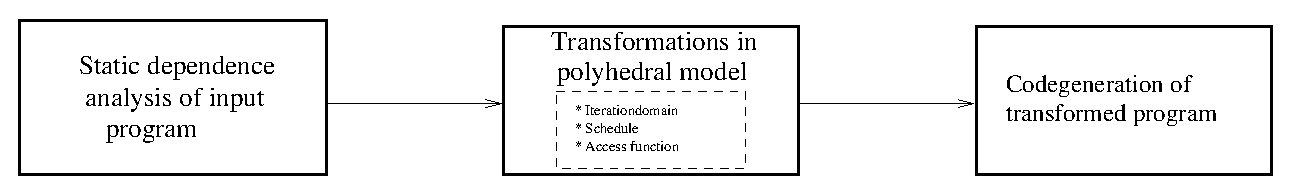
\includegraphics[width=1\textwidth]{images/poly_steps.eps}
  \caption{Transformation in polyhedral model}
\end{figure}

\subsection{Iteration Domain}
\subsection{The Schedule}
\subsection{Access function}


%%%%%%%%%%%%%%%%%%%%%%%%%%%%%%%%%%%%%%%%%%%%%%%%%%%%%%%%%%%%
% llvm
 \chapter{Introduction to LLVM}
\label{chap:llvm}
\section{What Is LLVM?}
LLVM is a virtual machine infrastructure that doesn’t provide any of the high-level features you’d find in something like the Java or .NET virtual machines, including garbage collection and an object model.

The basic design of LLVM is an unlimited register machine (URM), familiar to most computer scientists as a universal model of computation. It differs from most URMs in two ways:

\begin{itemize}
\item Registers are single-assignment. Once a value for a register has been set, it can’t be modified. This is a common representation in a lot of compilers, and has been since the idea was invented by an IBM researcher in 1985.
\item Each register has a type associated with it.
\end{itemize}

LLVM programs are assembled from basic blocks. A basic block is a sequence of instructions with no branches.

The low level virtual machine (LLVM) \cite{10.1109/CGO.2004.1281665} is a set
of tools and libraries to build a compiler. Constructed around a language and
platform-independent intermediate representation (IR) it provides
state-of-the-art analyses, optimizations and target code generation. Besides production
quality support for x86-32, x86-64 and ARM, there is target code generation for
the C programming language, various GPU accelerators or even hardware
descriptions.  There exist LLVM based static and just-in-time
compilers for nine of the ten most used programming languages \cite{tiobe11}.
Furthermore, there are OpenCL compilers developed by Apple, AMD and NVIDIA, as
well as various graphics shader compilers. Due to the modular structure, the
human readable IR and a set of helpful tools, development with LLVM is easy and
productive.

\section{The Intermediate Representation}

The core of LLVM is the intermediate representation (IR). Front ends compile code from a source language to the IR, optimization passes transform the IR, and code generators turn the IR into native code.
LLVM provides three isomorphic representations of the IR. The most common one used in examples is the assembly format, which looks roughly like an assembly language for a real machine (although with a few significant differences). A "Hello, world" program might look something like this:

\begin{verbatim}
  @.str = internal constant [12 x i8] c"hello world\00"

  define i32 @main() nounwind {
  entry:
    %tmp1 = getelementptr ([12 x i8]* @.str, i32 0, i32 0)
    %tmp2 = call i32 (i8*, ...)* @printf( i8* %tmp1 ) nounwind
    ret i32 0
  }
\end{verbatim}
First is a constant string, @.str. This has two qualifiers, internal and constant, which are the equivalent of static const in C. It then has a type. The square brackets signal that it’s an array; in this case, an array of 12 8-bit integers.
The main function doesn’t contain any branches, so it’s a single basic block. The label entry: indicates the start of the basic block, and the final instruction, ret, indicates the end. Every basic block is terminated with some kind of flow-control instruction. The ret instruction means return; in this case, returning 0 as a 32-bit integer. The type specified by the ret instruction and the return type specified in the function definition must match, or the IR will fail to validate.
Above the return instruction is a call to printf. Again, note the type signatures everywhere. The printf function’s return and argument types are given explicitly, and the types of the arguments are also listed. nounwind on the end indicates that this function is guaranteed not to throw an exception, which can be used in optimization later.

The first instruction in this basic block is one that most difficult one to grasp. Most programming languages (certainly, all Algol-family languages) contain some data structures that are accessed via offsets from their starts. A lot of CPUs include complex addressing modes for dealing with them. The getelementptr instruction (often referred to as GEP) provides something that can easily map to both.
The first argument is a complex type, in this case our global string variable. Note that, although the string is declared as an array type, when you reference it you actually get a pointer to that array. Our printf statement wants a pointer to an i8, but we have a pointer to an array of i8s. The remaining arguments to our GEP instruction are element offsets. The first dereferences the pointer, to give an array. The second then gets a pointer to the 0th element in the array. This instruction can get pointers to any element in an arbitrarily-complex data structure.
The GEP instruction does not dereferences the pointer. The GEP instruction just calculates offsets. When given all zero arguments, as in this example, all it’s really doing is casting a pointer to another type, which will emit no code in the final code-generation phase. This instruction could be replaced by a cast instruction that would simply change the pointer types. Both are semantically valid in this instance, but the GEP instruction is safer because it will validate the types.

While this representation of the IR is the one you’re likely to see most often, it’s not the most commonly used format. When generating IR, it’s common to use a set of C++ classes that represent it and provide convenience methods for constructing it. Intermediate values then are referenced simply as pointers to llvm::Value objects, rather than by name. Most of the time, the IR is used; but when being generated, transformed, or emitted, the C++ representation is used.

The final representation is the bitcode, a very dense binary Format used to transfer LLVM IR between components in different address spaces. When using LLVM tools connected by pipes, the bitcode is sent between them. It can also be serialized to disk and loaded later.


%%%%%%%%%%%%%%%%%%%%%%%%%%%%%%%%%%%%%%%%%%%%%%%%%%%%%%%%%%%%
% polly
\chapter{Polly - Pollyhedral optmizations in LLVM}
\documentclass[a4paper,10pt]{article}
%\usepackage{fancyvrb,relsize}
\usepackage{graphicx}
\usepackage[margin=2.25cm]{geometry}
\title{Learning Polly}
\date{7 November 2010}
\author{Raghesh A (cs09m032)}
\linespread{1.3}
\setlength{\parindent}{0pt}
\setlength{\parskip}{1ex plus 0.5ex minus 0.2ex}
\begin{document}

\maketitle

\section{Pre-requesites}
\begin{itemize}
\item SSA - \emph{http://en.wikipedia.org/wiki/Static\_single\_assignment\_form}
\item Dominators - \emph{http://en.wikipedia.org/wiki/Dominator\_\%28graph\_theory\%29}
\item Common Optimizations - \emph{http://en.wikipedia.org/wiki/Static\_single\_assignment\_form}
\begin{itemize}
\item constant propagation
\item  sparse conditional constant propagation
\item  dead code elimination
\item  global value numbering
\item  partial redundancy elimination
\item  strength reduction
\item  register allocatio
\end{itemize}
\end{itemize}
\section{The -polly-print Option}

Source File: SCoPPrinter.cpp

Generates the input datastructure as needed by cloog. Ulitmately call cloog to generate the C like code and 
out put that to stdout using c.pprint function.


\section{The -polly-scops Option}

Source File: SCoPInfo.cpp

\section{Overview}

The \emph{SCoPInfo} class defined in \emph{SCoPInfo.h} has a variable \emph{scop} of type \emph{SCoP *}. This is 
initialized by \emph{SCoPInfo::runOnRegion} function by calling the constructor for \emph{SCoP}. Inside the \emph{SCoP}
constructor after filling up the necessary arguments \emph{SCoP::buildSCoP} function is called. Details about this
important function is explained in the next section.

\subsection{The buildSCoP function}

\subsection{Arguments}
\begin{itemize}
\item TempScop: A helper class for remembering the parameter number and the max depth in this SCoP, and others context.
\item Region:  A Region is a connected subgraph of a control flow graph that has exactly
two connections to the remaining graph. It can be used to analyze or
optimize parts of the control flow graph.

A  \emph {simple Region}  is connected to the remaing graph by just two

An \emph  {extended Region}  (or just Region) is a subgraph that can be
transform into a simple Region. The transformation is done by adding
BasicBlocks that merge several entry or exit edges so that after the merge
just one entry and one exit edge exists.

The \emph Entry of a Region is the first BasicBlock that is passed after
entering the Region. It is an element of the Region. The entry BasicBlock
dominates all BasicBlocks in the Region.

The \emph Exit of a Region is the first BasicBlock that is passed after
leaving the Region. It is not an element of the Region. The exit BasicBlock,
postdominates all BasicBlocks in the Region.

A \emph {canonical Region}  cannot be constructed by combining smaller
Regions.

Region A is the \emph parent of Region B, if B is completely contained in A.

Two canonical Regions either do not intersect at all or one is
the parent of the other.

The \emph {Program Structure Tree} is a graph (V, E) where V is the set of
Regions in the control flow graph and E is the \emph parent relation of these
Regions.

\emph {Note: To get the regions in a program: opt -regions -analyze anyprogram.ll}

Example:
\begin{verbatim}
A simple control flow graph, that contains two regions.

        1
       / |
      2   |
     / \   3
    4   5  |
    |   |  |
    6   7  8
     \  | /
      \ |/       Region A: 1 -> 9 {1,2,3,4,5,6,7,8}
        9        Region B: 2 -> 9 {2,4,5,6,7}
\end{verbatim}

\item NestLoops: Todo
\item Scatter: Todo
\item LoopInfo: Todo
\item ScalarEvaluation: Todo
\end{itemize}

\section{Exercise 1: Analysing polly to detect read access statements}

This experement had a very short life since polly already does the dead code elemination of read access statements. Any way the work done for this explained in the next two subsections and reason for dropping this is explained in the third subsection.
\subsection{Adding a Newpass: Insert a function call}
The following code implements an optimization pass that can be invoked via "opt" with the flag "-insertcall". This pass inserts the function "void functionName(int)" into the symbol table of the program and inserts a call to this function before the terminator instruction of the last bask block of every function of the program. 

%\begin{Verbatim}[fontsize=\relsize{-1}, 
%                 frame=single, 
%                 fontfamily=courier,
%                 fontseries=b
%                 ]
\begin{verbatim}
#include "llvm/Pass.h"
#include "llvm/Function.h"
#include "llvm/Module.h"
#include "llvm/CallingConv.h"
#include "llvm/DerivedTypes.h"
#include "llvm/InstrTypes.h"
#include "llvm/Constants.h"
#include "llvm/Instructions.h"
using namespace llvm;
namespace {
    struct InsertCall : public FunctionPass {
        Constant *fcall;
        public:
        static char ID; // Pass identification, replacement for typeid
        InsertCall() : FunctionPass(&ID) {}
        virtual bool doInitialization(Module &mdl) {
            fcall = mdl.getOrInsertFunction("functionName",
                    /* return type */     Type::getVoidTy(mdl.getContext()),
                    /* actual 1 type */   IntegerType::get(mdl.getContext(), 32),
                    NULL);
            if( !fcall ){
                cerr << "### Error: fcall is NULL\n" << std::endl;
            }
            // Set the calling convention to C, so we interoperate properly with C code.
            Function *tmp = cast<Function>(fcall);
            tmp->setCallingConv(CallingConv::C);
            return true;
        }
        virtual bool runOnFunction(Function &func) {
            Value *param;
            // Find the instruction before which you want to insert the function call
            Instruction *nextInstr = func.back().getTerminator();
            // Create the actual parameter for the function call
            param = ConstantInt::get(Type::getInt32Ty(func.getContext()), 555);
            // create and insert the function call
            CallInst::Create(fcall, param, "", nextInstr);
            // indicates that we changed the code
            return true;
        }
        // optimization passes should implement the following function to be efficient.
        // virtual void getAnalysisUsage(AnalysisUsage &AU) const {
        // }
    };
}
char InsertCall::ID = 0;
static RegisterPass<InsertCall> IC("insertcall", "This pass inserts a function call");
\end{verbatim}
%\end{Verbatim}
To add this pass to the existing polly do the following

\begin{itemize}
\item Edit the "CMakeLists.txt" file in "/home/raghesh/project/build/llvm/tools/polly/lib" directory
\item Add the line "Pollycde/PollyCde.cpp" to the macro named "add\_polly\_library"
\item Switch to directory "/home/raghesh/project/build/build" and type "make"
\end{itemize}
To run:
\begin{verbatim}
clang -S -emit-llvm file.c
opt -S -polly-cde file.s
\end{verbatim}
You can observe that a function call "call void @functionName(i32 555)" is inserted to end of each function 
just before the return statement

\subsection{A Simple Example with SCoP}
 
\begin{verbatim}
#include <stdio.h>
#define N 100
int A[N] = {0};
int B[N] = {0};
int C[N] = {0};
int main()
{
    int i = 0, j = 0, k = 0;
    for(i = 0; i < N; i++) {
        A[i] = j++;
        B[i] = j++;
        k = C[i];
    }
    return 0;
}
\end{verbatim}
To compile:
\begin{verbatim}
alias opt="opt -load /home/raghesh/project/build/build/lib/LLVMPolly.so"
clang -S -emit-llvm  cde_test1.c
opt -S -mem2reg -loopsimplify -indvars cde_test1.s $gt$ cde\_test1.preopt.ll
opt -polly-scops -analyze cde_test1.preopt.ll
\end{verbatim}
Observe that the scop is detected and the statements having write to array is detected.

\subsection{Why this attempt is dropped}
\emph{Note: I, you and we are to be changed. This section is made from mail threads}

The steps to do the exersice is first explained and some observations are made. In the end we foudn that the dead code elimination is already done

so first of all I propose you get a piece of code that is SCoP detected by polly. Just use the examples in test/Codegen/*.c for this.
                                                                                                                                                                       To verify the SCoP is detected by polly use either opt -polly-view, opt -polly-print or opt -polly-detect -analyze.
Here one example:

\begin{verbatim}
int A[N];
void foo() {
    int i;
    int j;
    for (i = 0; i < N; ++i)
    j = A[i];
    return;
}
\end{verbatim}

This SCoP should be detected by polly, and hopefully if you call opt -polly-scops -analyze the SCoP will have one statement which does read memory, but does not write to it. If you use opt -O3 all that code will probably be automatically removed by LLVM, however by just using opt -mem2reg and right afterwords calling polly, we should be able to translate it into the polyhedral model and do the same dead code elimination inside polly.

This is no useful optimization as LLVM can do the same, but it should be easy.

So the way to go is to do:
1. Check if the above SCoP is detected.
2. See what its polyhedral representation looks like "opt -polly-scops -analyze"
3. The information should show one statement, that does read memory, but that does not write memory.
4. You write a LLVMPass that requires the SCoPInfo analysis and prints a list of all SCoPStmts in the detected SCoP that do not have any write accesses. 


Right now I am trying to print the statements with read access inside SCoPInfo.cpp itself, before making it a separate pass(to know I am able to get the information).

I am using the following code 


\begin{verbatim}

#include <stdio.h>
#define N 100

int A[N] = {0};
int B[N] = {0};
int C[N] = {0};
int main()
{
    int i = 0, j = 0, k = 0;

    for(i = 0; i < N; i++) {
        A[i] = j++; // S1
        B[i] = j++; // S2
        k = C[i];   // S3
    }   

    return 0;
}

\end{verbatim}

I observed that when the statements S1 and S2 are commented out the function "isTrivialBB" inside "buildSCoP" always returns true and nothing is inserted into the "Stmts" vector. If S1 or S2 is there it fails and the statement is inserted. Why does this happen?

My plan is that if I can push the statement S3 (statement with read access) into the vector, I can retrieve S3 inside "MemoryAccess::print". Here I could see the statements with write access are retrieved and printed. So I guess similar approach should be possible for read statements also.

This maynot be the right method. I just want to know that whether my understanding is correct.

Basically as explained in my previous mail I have made an attempt to print the "statements with read access" in the same way "statements with write access" are printed. The Write statements are printed in MemoryAccess::print and there is an isRead() function call. I thought that this function checks whether the current statement is having only a read access or not. But I think my understanding is wrong.

I need to look a little bit close into this example. I think you found one of the not so nice parts of polly.

By calling -polly-scops (which is just an analysis) we also schedule a transformation pass -polly-independent, which prepares the SCoP for us.

This is not obvious and should be changed. As a short term solution I propose you do this:

opt -polly-independent file.ll -S -o file.preopt.ll
opt -polly-scops file.preopt.ll

This should du the same, but you can see the changes -polly-independent did. So to figure out why the read is not available you can have a look at:

opt -view-cfg file.preopt.ll

and see if the expected store/load instructions are in the CFG.

While having a short look at this example, I had the impression -polly-independent remove the load. However I am not sure. This needs some more work.
I just had a look and it seems -polly-independent is already dead code eliminating the read accesses.

You can see it yourself by calling
"opt -polly-scops -view-cfg file.ll"

of

"opt -polly-scops -analyze file.ll"

There is no read / load statement left.

I think this project will not work as the read statements are already deleted.

So this attempt is dropped
\section{Exercise 2: OpenMP Code Generation Project}

\emph{Note: I, you and we are to be changed. This section is made from mail threads}

In light of the dropped attempt Tobias has suggested to look into this project. The details are explained below.
To start I attached you a small example "single\_loop\_openmp.c".

This function can be compiled by gcc in two ways. Either with or without openmp:\\
$>$ llvm-gcc -O3 single\_loop\_openmp.c\\
$>$ time ./a.out\\
real    0m4.170s\\
user    0m4.140s\\
sys     0m0.020s\\
$>$ llvm-gcc -O3 single\_loop\_openmp.c -fopenmp\\
$>$ time ./a.out\\
real    0m1.799s\\
user    0m6.410s\\
sys     0m0.030s\\

As you see openmp parallelism gives a nice benefit, but requires the openmp pragma comments.

We can now try to do this automatically using Polly.

First we need to detect the loop nest (I assume for all this you use dragonegg as llvm-gcc. We use dragonegg as it has the best openmp support)

\# Get LLVM-IR\\
    $>$ llvm-gcc -fplugin-arg-dragonegg-emit-ir -S single\_loop\_openmp.c\\
\# Canonicalize the SCoP\\
    $>$ opt -mem2reg single\_loop\_openmp.s -S > single\_loop\_openmp.preopt.ll\\
    $>$ opt -polly-print single\_loop\_openmp.preopt.ll -disable-output\\
    In function: 'single\_loop\_openmp' SCoP: 7 => return:
\begin{verbatim}    
    for (c2=0;c2<=10239999;c2++) {
         %"3"(c2);
          for (c4=0;c4<=400;c4++) {
                 %"4"(c2,c4);
                  }
    }
\end{verbatim}
\# If we now codegenerate this one normally, we generate a sequential
\# loop, without OpenMP\\
$>$ opt -polly-codegen single\_loop\_openmp.preopt.ll

\# However I just committed some infrastructure to start the work on
\# OpenMP parallel loops. Using the command line option we can mark
\# certain loops as parallel\\
$>$ opt -polly-codegen -polly-codegen-parallel=c2 \
                                              -debug-only=polly-codegen single\_loop\_openmp.preopt.ll\\
                                              Loop with header: polly.loop\_header is parallel

                                              This code was committed to lib/CodeGeneration.cpp. It changes codegen(struct clast\_for *f) such that a function is\_parallel() decides if an openmp parallel loop should be constructed or a normal sequential loop should be constructed.

                                              Lets assume the is\_parallel function knows what it is doing (we give it the information using the command line). In that case we need now to change the codegeneration a little, such that openmp parallel code is generated.

                                              What exactly needs to be changed is something I do not know yet. ;-)

                                              The first step will be to find out what a \# pragma omp parallel for does on the LLVM IR level.

                                              You can see the difference by calling\\
                                              $>$ llvm-gcc -fplugin-arg-dragonegg-emit-ir -S single\_loop\_openmp.c \
                                                   -o without-openmp.ll\\
                                              $>$ llvm-gcc -fplugin-arg-dragonegg-emit-ir -S single\_loop\_openmp.c \
                                                        -fopenmp -o without-openmp.ll\\

                                                        And looking at the LLVM-IR output of both statements.

                                                        Further documentation can be found here:
                                                        http://gcc.gnu.org/onlinedocs/libgomp/Implementing-FOR-construct.html\#Implementing-FOR-construct

                                                        Be careful just the first example applies for the moment:


\begin{verbatim}
#pragma omp parallel for
for (i = lb; i <= ub; i++)
body;
------------------
becomes
------------------
void subfunction (void *data)
{
    long _s0, _e0;
    while (GOMP_loop_static_next (&_s0, &_e0))
    {
        long _e1 = _e0, i;
        for (i = _s0; i < _e1; i++)
            body;
    }
    GOMP_loop_end_nowait ();
}

GOMP_parallel_loop_static (subfunction, NULL, 0, lb, ub+1, 1, 0);
subfunction (NULL);
GOMP_parallel_end ();
------------------
\end{verbatim}
\section{The codegenForSequential Function}
We have to write the codegenForOpenMP function. So learning codegenForSequential is a prerequisite for that.
\subsection{Builder}
The Builder specifies the current location to code generate at
\subsection{Stride}
The number by which the loop iv is incremented after every iteration.
\subsection{createLoop Function}
This creates the code for a single loop. If we have a nested loop this function is called recursively.
There are four parts for the body of the function which are PreheaderBB, HeaderBB, BodyBB, AfterBB. 
PreHeaderBB is the Current BB and the HeaderBB is added to the PreHeaderBB. 
Using addNewBlock function basic blocks are inserted as the child of other basic blocks. Using 
Create<InstructionName> Function New instructions are created. These instructions are appended to a 
particular basic block using SetInsertPoint function. 


\section{Jumping into coding}

Understood the flow and now starting to code

\subsection{Adding prototype and call to GOMP\_parallel\_end}
The pseudo code is given below
\begin{verbatim}
codegenForOpenMP() {
    createSubFunction()
    createLoopForOpenMP()
}

createLoopForOpenMP() {
    Insert_Call_corresponding_to_GOMP_loop_static()
    Insert_Call_subfunction()
    Insert_Call_corresponding_to_GOMP_parallel_end()
}
\end{verbatim}
very simple instruction to add is an instruction that allocates some space in memory.

\begin{verbatim}
void codegenForOpenMP(struct clast_for *f) {
    APInt Stride = APInt_from_MPZ(f->stride);
    PHINode *IV;
    Value *IncrementedIV;
    BasicBlock *AfterBB;
    Value *LB = ExpGen.codegen(f->LB);
    Value *UB = ExpGen.codegen(f->UB);

    =>  Value *AllocInstr = Builder->CreateAlloca(Builder->getInt32Ty(), 0,
            "TESTINSTRUCTION");

\end{verbatim}
When you call the modified code e.g. like this:

opt -polly-codegen -view-cfg -polly-codegen-parallel=c2

You should be able to find the TESTINSTRUCTION in the generated code. The next thing is to figure out how to insert a function call.

I propose to start with the call to:
call void @GOMP\_parallel\_end() nounwind

This is the easiest one, as it does not involve any parameters. This is also what I meant with "selfcontained". To insert this instruction you do not need to prepare anything else in polly, e.g. create the parameters first.

You probably need to create the definition of that function and than add the call to this function.

You may find some help in this tutorial:

http://llvm.org/docs/tutorial/LangImpl3.html\#exprs

Especially those functions (and their descriptions) should be useful to add the "call void @GOMP\_parallel\_end() nounwind" instruction:

Function *PrototypeAST::Codegen()
and
Value *CallExprAST::Codegen()

The code is added and now the following issues has to be verfied
1. What happens if there are two scops with openmp detected. Check whether two prototypes are added
2. What happens if there are scops in two different functions. Basic blocks links may be broken.

\subsection{Add check if OpenMP codegeneration is enabled}

Right now this is done with the following code. This is a method to add command line option to llvm.

\begin{verbatim}
static cl::opt<std::string>
    ParallelDimension("polly-codegen-parallel",
            cl::desc("The dimension which is parallel"), cl::Hidden,
            cl::value_desc("Name of dimension"),
            cl::ValueRequired, cl::init(""));
\end{verbatim}

Class Template named ParallelDimension is created and inside the IsParallelFor gets the value of
the iterator and compares it with the one specified by the user. This behaviour is to be changed
in a later implementation after performing the correct analysis.


\subsection{Adding OpenMP Subfunction}

So let's have a look at the OpenMP code:


\begin{verbatim}    
    ------------------
#pragma omp parallel for
    for (i = lb; i <= ub; i++)
        body;
------------------

    becomes

    ------------------
    void subfunction (void *data)
    {
        long _s0, _e0;
        while (GOMP_loop_static_next (&_s0, &_e0))
        {
            long _e1 = _e0, i;
            for (i = _s0; i < _e1; i++)
                body;
        }
        GOMP_loop_end_nowait ();
    }

GOMP_parallel_loop_static (subfunction, NULL, 0, lb, ub+1, 1, 0);
subfunction (NULL);
GOMP_parallel_end ();
------------------
\end{verbatim}

We already generated the call to "GOMP\_parallel\_end". I propose as a next step to create "subfunction" with an empty body and add the call to it right before the call to "GOMP\_parallel\_end".

Remember that subfunction takes one parameter called which is a of type "void *". It has no return value, which means it returns "void".

\emph{Note: Some Misunderstadings --- When the actual analysis is done, do we need to implement a seperate pass to detect whether there are OpenMP pragmas in the input file?. No, I propose not to work on OpenMP pragma support. It is not needed for automatic parallelization. We can (even if not implement at the moment) detect parallelism automatically. There is no need for any user added pragmas.}

\subsubsection{Getting unique name for subfunction}

Just get the name of the function "+" a string called ".omp\_subfunction". I believe llvm will take care itself that an unique number is appended.

\subsubsection{Adding subfunction body}

\begin{verbatim}

// Adding Subfunction body
//FN = M->getFunction("subfunction");
Constant* C = M->getOrInsertFunction("subfunction", Type::getVoidTy(Context),
        Type::getInt8Ty(Context)->getPointerTo(), NULL);
Function* SubFn = cast<Function>(C);
BasicBlock* SubFnBB = BasicBlock::Create(Context, "polly.subfn_entry", SubFn);;
DT->addNewBlock(SubFnBB, Builder->GetInsertBlock());

\end{verbatim}

The above code is just an outline for creating the subfunction body. Correct method is to be found.

\section{Adding GOMP\_parallel\_start}

\begin{verbatim}
Function *PsFN = M->getFunction("GOMP_parallel_start");
// Check if the definition is already added. Otherwise add it.
if (!PsFN) {
        // Creating type of first argument for GOMP_parallel_start.
        std::vector<const Type*> Arguments(1, Type::getInt8PtrTy(Context));
        FunctionType *FnArgTy = FunctionType::get(Type::getVoidTy(Context),
                        Arguments, false);
        PointerType *FnPtrTy = PointerType::getUnqual(FnArgTy);

        // Prototype for GOMP_parallel_start.
        std::vector<const Type*> PsArguments;
        PsArguments.push_back(FnPtrTy);
        PsArguments.push_back(Type::getInt8PtrTy(Context));
        PsArguments.push_back(Type::getInt32Ty(Context));
        FunctionType *PsFT = FunctionType::get(Type::getVoidTy(Context),
                        PsArguments, false);
        Function::Create(PsFT, Function::ExternalLinkage,
                        "GOMP_parallel_start" , M);
}
\end{verbatim}

\section{Using slightly different way to call libgomp}

I just looked again in the way we produce OpenMP library calls and realized that we model the library calls needed for a parallel for
that uses a static schedule:

\begin{verbatim}
#pragma parallel for SCHEDULE(static)
for (int i, ...
\end{verbatim}                

                which is the default used if SCHEDULE is not specified.

                Unfortunately this has two disadvantages.

                1. The user cannot specify at runtime what schedule technique he wants to be used.

                2. As the static schedule is simple, gcc does not emit function calls to calculate the lower and upper bounds of the induction variable in subfunction, but emits directly the LLVM-IR to calculate the lower and upper bound for a specific instance of subfunction.

                The second point complicates our life, as we would need to understand how gcc is calculating those bounds.

                I propose therefore to create code for a runtime switchable schedule technique.

                I attached an example plus the LLVM-IR produced by this example.

                The only thing we need to change in our current code is the call to
                GOMP\_parallel\_start. It needs to be replaced by a call to

                call void @GOMP\_parallel\_loop\_runtime\_start(void (i8*)* @single\_loop\_openmp.omp\_fn.0, i8* null, i32 0, i64 0, i64 10240000, i64 1) nounwind;

The arguments this call takes are:

GOMP\_parallel\_loop\_runtime\_start(subFunction, numberOfThreads, lowerBound, upperBound, stride);

numberOfThreads is always set to zero (this means it will be selected automatically).

The following code copied from codegenForSequential can be used to get
the other values.

\begin{verbatim}
APInt APStride = APInt_from_MPZ(f->stride);
Value *stride = ConstantInt::get(Builder->getInt64Ty(), APStride);
Value *lowerBound = ExpGen.codegen(f->LB);
Value *upperBound = ExpGen.codegen(f->UB);
\end{verbatim}

\section{Creating Body to Subfunction}

\subsection{Creating an Empty Body}

\begin{verbatim}
void addOpenMPSubfunctionBody(Function *FN, const clast_for *f) {
    LLVMContext &Context = FN->getContext();
    // Create a new basic block to start insertion into.
    BasicBlock *BB = BasicBlock::Create(Context, "entry", FN);
    // Store the previous basic block.
    BasicBlock *PrevBB = Builder->GetInsertBlock();
    // Add the return instruction.
    Builder->SetInsertPoint(BB);
    Builder->CreateRetVoid();
    // Restore the builder back to previous basic block.
    Builder->SetInsertPoint(PrevBB);
}


\end{verbatim}

\subsection{Linking basic blocks}

The basic structure of the basic block is described here. We have an header basic block(HeaderBB). This is set as a child to the previous basic Block(PrevBB). 
Now rest of the blocks are created as the child of HeaderBB as shown in the figure.
\begin{verbatim}
                ---------------
                |   PrevBB    |
                ---------------
                       |
                       |
                ---------------
                | HeaderBB    |
                ---------------
                   	/     \
                   /       \
        ---------------   ---------------
        |     BB1     |   |  ExitBB     |
        ---------------   ---------------
\end{verbatim}	
\section{Adding Nounwind and zeroext}
\begin{verbatim}
runtimeNextFN->addFnAttr(Attribute::NoUnwind);
\end{verbatim}

\section{Testing OpenMP Code Generation}

This section has some of the test cases to test the OpenMP code generation.

\subsection{Test Case 1}


\$opt -mem2reg  two\_loop\_openmp.s -S -enable-polly-openmp $|$ llc -o out.s\\
\$gcc out.s -lgomp\\
\$time ./a.out\\
real    0m1.479s\\
user    0m1.410s\\
sys     0m0.060s\\
\$opt -mem2reg -polly-codegen two\_loop\_openmp.s -S -enable-polly-openmp $|$ llc -o out.s\\
\$gcc out.s -lgomp\\
\$time ./a.out\\
real    0m0.073s\\
user    0m0.040s\\
sys     0m0.030s\\

This is on a dual core machine looking at the runtime we are getting a huge speedup.

\subsection{Test Case 2}

\$ opt -mem2reg -polly-codegen two\_loop\_openmp.s -S  $|$ llc -o out1.s\\
\$ gcc out1.s -lgomp\\
\$ time ./a.out\\
real    0m0.180s\\
user    0m0.084s\\
sys    0m0.088s\\
\$ opt -mem2reg -polly-codegen two\_loop\_openmp.s -S -enable-polly-openmp $|$ llc -o out.s\\
\$ gcc out.s -lgomp\\
\$ time ./a.out\\
real    0m0.090s\\
user    0m0.020s\\
sys    0m0.072s\\

\subsection{Test Case 3: Checking Correctness}

Use the following code to do this.

\begin{verbatim}
#include <string.h>
#include <stdio.h>
#define N 1024
float A[N];
void loop_openmp() {
    int i = 0;
#pragma omp parallel for schedule(runtime)
    for (i = 0; i < N; i++) {
        A[i] = i;
    }
}
float check_sum() {
    float sum = 0;
    int i = 0;
    for(i = 0; i < N; i++) {
        sum += A[i];
    }
    return sum;
}
int main () {
    memset(A, 0, sizeof(float) * N);

    loop_openmp();
    printf("sum = %f\n", check_sum());
    return 0;
}

clang -emit-llvm correctness.c -S
opt -mem2reg -indvars correctness.s -S > correctness.ll
opt -load /home/raghesh/project/build/build/lib/LLVMPolly.so -mem2reg -polly-codegen correctness.ll -S | llc -o out.s
gcc out.s -lgomp
time ./a.out
sum = 523776

real	0m0.001s
user	0m0.000s
sys	0m0.004s
opt -load /home/raghesh/project/build/build/lib/LLVMPolly.so -mem2reg -polly-codegen correctness.ll -enable-polly-openmp -S | llc -o out.s
gcc out.s -lgomp
time ./a.out
sum = 0

real	0m0.001s
user	0m0.000s
sys	0m0.000s

\end{verbatim}

The test case was a failure since we are getting sum = 0.

\subsubsection{Debugging}
1. Compare polly-openmp code with the one generated by llvm-gcc. I assume that llvm-gcc generated openmp code works fine. I will manually make changes, which is missing in our code(like zeroext, nounwind, etc). Could you please send me the .ll file generated by llvm-gcc for the correctness test case I sent?

2. If still the problem persists I will look into body of the subfunction and will examine it.

3. Use some debugging tools available in llvm for debugging the code in llvm-IR level. Is there any such tools? Can I use lldb?

\begin{verbatim}

I added a openmp version of the testcase. I propose to do the following.

Use llvm-gcc to create those two files

llvm-gcc -S -flto correctness.c -o correctness.noopenmp.s
llvm-gcc -S -flto -fopenmp correctness.c -o correctness.gccopenmp.s

opt -mem2reg -indvars correctness.noopenmp.s -S -o  \ correctness.noopenmp.ll
opt -mem2reg -indvars correctness.gccopenmp.s -S -o  \ correctness.gccopenmp.ll

opt -polly-codegen -enable-pollyopenmp correctness.noopenmp.ll -o \
			-S correctness.pollyopenmp.ll

			llc correctness.gccopenmp.ll
			gcc correctness.gccopenmp.s -o correctness.gccopenmp.exe
			./correctness.gccopenmp.exe

			llc orrectness.pollyopenmp.ll
			gcc correctness.pollyopenmp.s -o correctness.pollyopenmp.exe
			./correctness.pollyopenmp.exe

			I suspect we will still see, that the pollyopenmp code is not working. I propose now to work on the .ll files correctness.gccopenmp.ll and correctness.pollyopenmp.ll
			Create a third file correctness.merged.ll, that is just a copy ofcorrectness.gccopenmp.ll. Now try to transform this file step by step to correctness.pollyopenmp.ll and see when it's breaking.

\end{verbatim}
\subsubsection{Fix}

\begin{verbatim}

I think I have almost found the problem. I made the following changes.

Change 1
------------
Comparing the two files that you have suggested I observed that we have to jump back to the basic block bb1 from the branch polly.after_loop. We were jumping to exit. Now the result is fine.

And I made some minor changes.

Change 2
-------------
The prototype for GOMP_parallel_loop_runtime_start is changed from

declare void @GOMP_parallel_loop_runtime_start(void (i8*)*, i8*, i32, i64, i64, i64) nounwind

to

declare void @GOMP_parallel_loop_runtime_start(void (i8*)*, i8*, i32, i32, i32, i32) nounwind

The prototype for GOMP_loop_runtime_next is changed from

declare i8 @GOMP_loop_runtime_next(i64*, i64*) nounwind

to

declare i8 @GOMP_loop_runtime_next(i32*, i32*) nounwind

I think the prototype change may not work always since some time we need may need i64 type. We have to handle this

This is fixed by adding a command line option -set-polly-openmp32 which changes the declaration if its a 32 bit machine.
Change 3
-------------
I have added the required nounwind and zeroext attributes

Please note that the changes made are manual changes to .ll file. Not in code.
\end{verbatim}

\subsection{Test Case 4: Checking correctness with nested loops}

This is test the correctness of nested loops.

It fails

\subsubsection{Debugging}

find attached a script and input files. I could see the result is wrong even when just llvm-gcc is used with openmp enabled. When openmp pragma is enabled for both the loops the result is correct.

Test 1: Clang for correctness\_large.c

sum = 50.000000

Test 2: With Polly openmp for correctness\_large.c

sum = 73.000000

Test 3: gcc openmp for correctness\_large\_openmp.c

sum = 46.000000

Test 4: gcc openmp for correctness\_large\_openmp.c with pragma for both loops

sum = 50.000000

\begin{verbatim}

correctness_large.c
-------------------
#include <stdio.h>
#define N 5
double A[N];
void loop_openmp() {
  for (int i = 0; i < N; i++) {
    for (int j = 0; j < 5; j++)
      A[i] += j;
  }
}
float check_sum() {
  float sum = 0;
  for(int i = 0; i < N; i++) {
    sum += A[i];
  }
  return sum;
}
int main () {
  memset(A, 0, sizeof(float) * N);
  loop_openmp();
  printf("sum = %f\n", check_sum());
  return 0;
}
correctness_large_openmp.c
---------------------------
#include <string.h>
#include <stdio.h>
#define N 5
double A[N];
void loop_openmp() {
  int i = 0, j = 0;
#pragma omp parallel for schedule(runtime)
  for (i = 0; i < N; i++) {
    for (j = 0; j < 5; j++)
      A[i] += j;
  }
}
float check_sum() {
  float sum = 0;
  int i = 0;
  for(i = 0; i < N; i++) {
    sum += A[i];
  }
  return sum;
}
int main () {
  memset(A, 0, sizeof(float) * N);
  loop_openmp();
  printf("sum = %f\n", check_sum());
  return 0;
}
correctness_large_openmp2.c
---------------------------
#include <string.h>
#include <stdio.h>
#define N 5
double A[N];
void loop_openmp() {
  int i = 0, j = 0;
#pragma omp parallel for schedule(runtime)
  for (i = 0; i < N; i++) {
#pragma omp parallel for schedule(runtime)
    for (j = 0; j < 5; j++)
      A[i] += j;
  }
}
float check_sum() {
  float sum = 0;
  int i = 0;
  for(i = 0; i < N; i++) {
    sum += A[i];
  }
  return sum;
}
int main () {
  memset(A, 0, sizeof(float) * N);
  loop_openmp();
  printf("sum = %f\n", check_sum());
  return 0;
}

\end{verbatim}

\subsubsection{Fix}

To fix it you can do not need two openmp loops, but you need to declare the inner induction variable private or declare it inside the inner loop. Otherwise it will be shared and everything becomes incorrect

\begin{verbatim}
void loop_openmp() {
   int i = 0, j = 0;
    #pragma omp parallel for schedule(runtime) private(j)
    for (i = 0; i < N; i++) {
         for (j = 0; j < 5; j++)
                A[i] += j;
          }
}

void loop_openmp() {
   int i = 0;
    #pragma omp parallel for schedule(runtime)
    for (i = 0; i < N; i++) {
         int j;
            for (j = 0; j < 5; j++)
                   A[i] += j;
             }
}
\end{verbatim}

I looked into this bug a little. After some investigation I realized that openmp is describing the loops as "$<$" and we describe the loops as "$<=$". By adapting the number of loop iterations at two places this bug can be fixed. I attached a patch that does this. It might need some adaption to compile on 32bit. Can you verify it works for you?
\subsection{Test Case 5: Check whether the loops are split into different cores}
\subsection{Test Case 6}

Support openmp loops, that are not the outermost loops. Those loops
need the values of the surrounding induction variables in the openmp
subfunction.

\subsection{Test Case 7}

Support parameters. Those need also to be passed to the subfunction.

\section{Adding Test Cases to Polly}
So to add the tests you should use test/create\_ll.sh to create .ll files of the .c files. And add
the relevant check that add least check the relevant openmp
function calls are added.

And finally you should check if the tests are executed and pass
by calling:

make polly-test

It would be good to send out patch for this first.

\section{OpenMP Code Generation for inner loops}

So far we have created OpenMP code for only outer loops. Next step is to do it for inner loops. For that we have to do the following

Support openmp loops, that are not the outermost loops. Those loops
need the values of the surrounding induction variables in the openmp
subfunction.

You will need to pass the values of the outer induction variables in a structure to the subfunction. I propose to start with a structure to which you add the current values of all surrounding ivs.

We have to handle the following issues

1. To see the the scenario which we have to handle see the following code. 
\begin{verbatim}
  for (i = 0; i<  N; i++)
  #pragma omp parallel for schedule(runtime)
    for (j = 0; j<  5; j++)
     A[i] += j;

\end{verbatim}

We have to create OpenMP code similar to the one generated by llvm-gcc with -fopenmp enabled.

In the above example the inner most loop is not parallel due the following reason.

The OpenMP pragma is invalid at this place. The code that is executed in the innermost loop is:

\begin{verbatim}
A[0] = A[0] + 0; // Iteration 0
A[0] = A[0] + 1; // Iteration 1
A[0] = A[0] + 2; // Iteration 2
A[0] = A[0] + 3; // Iteration 3
A[0] = A[0] + 4; // Iteration 4
\end{verbatim}
Every iteration works on the same memory. Iteration 1 needs therefore Iteration 0 to be finished before it can read the value of A[0].
The inner loop is therefore not parallel. Try something like this, where the inner loop is parallel, but the outer loop is not.


\begin{verbatim}
for (j = 0; j <  5; j++)
 #pragma omp parallel for schedule(runtime)
    for (i = 0; i <  N; i++)
            A[i] += j;
\end{verbatim}
2. With the current implementation all the outermost loops which are
detected as SCoP are converted to OpenMP parallel loops. But, if my
understanding is correct there is no way to say that "Dont parallalize
the outermost loop, but do it for innerloop". How do we specify this?
Earlier we had an option -polly-codegen-parallel=c4 which can be used to
specify the particular inner loop. How do we automate this?

This is already done (but may still have some bugs):

\begin{verbatim}
void codegen(const clast_for *f) {
  if (Vector && isInnermostLoop(f) && isParallelFor(f)) {
    codegenForVector(f);
  } else if (OpenMP && !parallelCodeGeneration && isParallelFor(f)

\end{verbatim}

Polly checks if a loop is parallel and uses OpenMP for the outermost loop that is parallel. So the way to not parallelize the outermost loop is to create a test case, where the outermost loop can not be executed in parallel, because it is carrying dependencies (This means parallelizing it would create invalid code).

You may want to add debugging code to inform about this decision.

\subsection{Implementation}

I have identified the following logical steps to implement this.
\begin{itemize}
\item Creating the llvm structure to store arguments(induction variables
  of outer loop) to the subfunction.
\item Store required values into the structure.
\item Changing the signature of the prototype and call of
GOMP\_parallel\_loop\_runtime\_start as

void @GOMP\_parallel\_loop\_runtime\_start(void (i8*)* @subfunction, i8*
  \%.omp\_data, i32 , i32 , i32 , i32 )

\item Changing the signature of the prototype and call to subfunction  as

void @subfunction(i8* \%.omp\_data)

\item Make the corresponding changes in the subfunction body.
\end{itemize}

Agreed. You should probably store the contents of CharMap in this struct.

Why do you need to change the prototype? Is it not sufficient to change
the parameter for the second argument. Such that a pointer to your struct is passed instead of a NULL pointer as we do it right now.


4. Changing the signature of the prototype and call to subfunction  as

void @subfunction(i8* %.omp_data)

I think the signature should already be alright. We already require one pointer to be passed to the subfunction.


5. Make the corresponding changes in the subfunction body.

You should read the values from the struct and update CharMap to point to the new values, instead of the original onces in the main function.

> I have identified the following logical steps to implement this.
>
> 1. Creating the llvm structure to store arguments(induction variables
    > of outer loop) to the subfunction.

In the attached patch I have written an outline for a function to
create the structure to store the subfunction parameters. I think we
can use the same structure to store any variable defined outside the
particular inner loop.

Inside the function we have to do the following.

Examine the body of the for loop to find the variables referred which
are defined outside the loop. Add the types of those to the
subfunction parameter structure. I am thinking to use following for
loop to examine the body of the  for loop(which is the current SCoP)
\begin{verbatim}
for (Scop::iterator SI = S->begin(), SE = S->end(); SI != SE; ++SI) {
      ScopStmt *Stmt = *SI;
       }
\end{verbatim}
But I couldn't find a method to examine the SCoP statements. How Can I do that?

  Or is there any other method without iterating through the SCoP statements ?

I believe it is enough to store the content of the CharMap in that struct. Just iterate over the CharMap and store all its content in the order it appears in the CharMap.

This part is not done in the code yet. If there is no variables
referred we just pass null as argument to subfunction(as we did
    earlier.) At that time no structure is created.


I propose not to think about the variables referred in subfunction, but just the values available in CharMap. Only if no value is in CharMap we should pass an empty structure.


have made some progress. But the patch attached is still incomplete.
Need your comments to move forward.

Till now I am able to store all the parameters in CharMap to the
structure. I feel some improvements can be done. But not sure how?

1. Can we put the two for loops together so that its possible to
create the structure and add the values to the structure at the same
time. Now in the first for loop I am iterating through charMap to
decide the type of the structure and in another for loop the values
are stored into the structure.

I do not think so. It will be difficult to insert something into a structure that does not yet exist.


2. Please note I commented about another way to get the unique name
for the structure. Is the current way fine?

  Probably  not for all cases (as we may need multiple of those structures in a function. Maybe something is already doing some magic. So let's leave it like this for the moment.

      I believe the following steps have to be done to complete this

      1. In addOpenMPSubfunctionBody() read the structure and load the
      values into variables having the same I thinnames in CharMap. Is it correct?

      I would just load the values from the structure and update CharMap (temporarily - keep a copy and insert the original values later).


      2. Now I commented addOpenMPSubfunctionBody(). I will remove the
      comment once step \#1 is done. As you said there is no harm in calling
      the functions in the following order

      addOpenMPSubfunctionBody()
      addOpenMPSubfunctionParams()

      Does this order still work for step \#1. I suppose you need the created structure to read from it?


      I have attached the .c and .ll files also.


I found another issue when we have nested loops. This is there even if
the inner loop doesn't have any variable references defined outside. I
think I have to fix this before moving forward.

The input files are attached. I am getting the following error with
the following command
\begin{verbatim}
> clang -emit-llvm innerloop.c -S
> opt -mem2reg -polly-codegen -enable-polly-openmp innerloop.s  -set-polly-openmp32 -S > innerloop.ll
Instruction does not dominate all uses!
 %polly.loopiv = phi i32 [ 0, %pollyBB ], [ %polly.next_loopiv,
  %polly.loop_body ]
     %8 = mul i32 1, %polly.loopiv
     Broken module found, compilation aborted!
     Stack dump:
     0.      Program arguments: opt -load
     /home/raghesh/project/build/build/lib/LLVMPolly.so -mem2reg
     -polly-codegen -enable-polly-openmp innerloop.s -set-polly-openmp32 -S
     1.      Running pass 'Function Pass Manager' on module 'innerloop.s'.
     2.      Running pass 'Module Verifier' on function '@loop_openmp.omp_subfn'
     Aborted
     \end{verbatim}
The problem is with linking the basic blocks.

  The issue is not there with the following loop
\begin{verbatim}
  for (int i = 0; i<  N; i++) {
    for (int j = 0; j<  N; j++) {
      A[i] += j;
    }
  }
\end{verbatim}
That is there is no problem if the outer loop itself is detected as
  SCoP. If the inner loop is detected as SCoP basic block links are
  broken.


  This is because we do not yet support the parallelization of inner loops. The code in the loop will refer to "i" which is now in a completely different function, which obviously is not correct. To see
  the produced LLVM-IR you can use -disable-verify.

  Yes. It refers to branches and variables which is not defined in the
  subfunction. I will fix that.


  I believe this should work out of the box after you pass the parameters using the struct.


  Is there any way to view the LLVM-IR produced through gdb?


  Sure. $->$dump() for a basic block or a value and $->$viewCFG for a function.

\subsection{Adding Domination Check}  
I am trying to iterate through the struct members while reading the
	struct. I have attached two patches. One with domination check and
	another without it. For testing purpose I am still using CharMap to do
	the following.

	OMPCharMap[I->first] = Builder->CreateLoad(loadAddr);

This is to be changed. But I am not sure how to do it. Can you suggest a method?

	And I am trying to execute the following loop where the inner loop is
	not parallel.
\begin{verbatim}
	for (int i = 0; i < N; i++) {
		for (int j = 0; j < N; j++) {
			A[j] += j;
		}
	}
\end{verbatim}

This is because the inner loop is a sequential loop and it will try to
	access OMPCharMap to get some values. But it doesn't have any value.
	That is still we need all the values of CharMap to be copied to
	OMPCharMap. I tried to reset the it to CharMap just before calling
	codegenForSequetial in isParallelFor function.

	I tried different ways to fix it. But couldnot succeed.

	In the second patch, though it's not the right way, I removed the
	domination check and iterate over CharMap and it works.

Ok. So the reason this does not work is probably that we do not update the dominance information correctly. I believe the right fix is to make sure we update it correctly. Can you run

opt -polly-codegen -verify-dom-info

I believe it will fail, and we should try to fix it.

Yes. This fails even for a single loop like


\begin{verbatim}
for(i = 0; i < N; i++)
	   A[i] = 1;
\end{verbatim}

\subsubsection{Debugging}
While debugging one thing I noticed is that in the dominator tree for
	the caller of subfunction, entire dominator tree of subfunction is
	duplicated. Attached the dominator trees. I think we have to remove
	this.

	This happens because in the subfunction body PrevBB is added as the
	parent of HeaderBB. I think we should have different domination trees
	for different functions. How can I create a separate one for the
		subfunction?

			I am not sure this will fix the issue. But anyway this is to be done.

The problem is probably that we create a new subfunction in a RegionPass. This is something that is probably not valid. It might be helpful to look e.g. at the loop extractor pass and see how they extract a loop into a new function. Maybe the use a module pass.

A quick fix might be to not rely on valid dominator information in the codegeneration pass, however we than need another way to derive what elements need to be added to the structure.                                                                                                                                                                                                              I am fine with this. I believe however that it will be difficult to generate correct dominator information for the subfunction as long as lib/CodeGeneration is a RegionPass. As I do not like to promote it to a module pass we need to work something out.

I am interested to hear how you plan to solve the dominator issue.

\section{Support for lastprivate and reduction attributes in Polly}

Consider the following code segment

\begin{verbatim}
int loop1_openmp() {
    int i = 0, k = 0;;
    for (i = 0; i <= N; i++) {
             A[i] = 0;
    }
    return i;
}
\end{verbatim}


The corresponding .ll files generated for the above cases with polly and llvm-gcc are atttached. It is observed that llvm-gcc add the iteration variable to the parameter structure to the subfunction and somehow(to be examined how) they reload 'i' and return the correct value. But since we are creating the parameter structure from CharMap(where iteration variable is not there) an empty structure is created. How can we solve this problem?

Also consider the following code segment

\begin{verbatim}
int loop1_openmp() {
    int i = 0, k = 0;;

    #pragma omp parallel for schedule(runtime) lastprivate(i) reduction(+: k)
    for (i = 0; i <= N; i++) {
             A[i] = 0;
	     k++;
    }
    return i + k;
}
\end{verbatim}

With Polly this particular loop is not detected as SCoP. Will this be detected as SCoP in future?

\section{Bench Mark}
1. OpenMP Code Generation(Testing real programs)

	You might have a look at:

	http://hpc.cs.tsinghua.edu.cn/research/cluster/SPEC2006Characterization/auto\_para.html

	Some like cactusADM have very nice results. Do you have access to SPEC2006? In case you have I suggest to try to optimize cactusADM.
	This will be a larger project, but very worthwhile. If you don't have,
	     cactusADM is actually open source. You can probably download it
		     on cactuscode.org



Refer http://en.wikipedia.org/wiki/Benchmark\_\%28computing\%29

\section{Actual Analysis to Detect Parallel Loops}

I just committed some changes to polly that add detection of parallel loops. So instead of using -polly-codgen-parallel=c2, just use -polly-codgen-parallel=true to enable OpenMP code generation.The functionality I added is not a complete new pass, buta new function added to the dependency analysis. You can see the changes needed in the last commit. "git log -p"



\section{Replacement for -polly-print option}

The -polly-print option to dump the cloog output has been removed. Now we can use the following command

\emph{opt -polly-cloog -analyze two\_loop\_openmp.ll}

If there is too much information use

\emph{opt -polly-cloog -analyze two\_loop\_openmp.ll -q}

\section{To See list of optimization passes}

OPT documentation mentions optimization options -O1,-O2 and -O3 etc.
(I am using -O0, no optimizations). The documentation does not tell
 you what optimizations are included in each option.  It says they are
 same as gcc.  gcc dodoc is not of much help either.  Where can I find
 this information.

Just call

opt -O3 -debug-pass=Arguments program.ll

which prints the list of passes executed.

\section{Printing Strings in llvm}

\begin{verbatim}
std::string output;
raw_string_ostream OS(output);
const std::string &Name = F->getNameStr();
OS << "In function: '" <<  Name+".omp_subfunction" << "\n";
fprintf(stdout, "%s", OS.str().c_str());

\end{verbatim}
\section{Preparing Application for GSOC 2011}
Is it possible for you to mentor me in contributing to Polly? If so I
can contribute to some of the following projects

Sure. Just include my name in your application and we will be set. However I cannot guarantee it will be accepted. This will be elected by all LLVM mentors.

1. OpenMP Code Generation(Testing real programs)

	You might have a look at:

	http://hpc.cs.tsinghua.edu.cn/research/cluster/SPEC2006Characterization/auto\_para.html

	Some like cactusADM have very nice results. Do you have access to SPEC2006? In case you have I suggest to try to optimize cactusADM.
	This will be a larger project, but very worthwhile. If you don't have,
	     cactusADM is actually open source. You can probably download it
		     on cactuscode.org

		     2. Porting Polly to various targets.(not sure is it a valid one)

		     Very valid.

		      3. Profiling in Polly

		     I also like this idea. Developing some way to understand how much time is spent in which SCoP.

		      4. Contributing to Ether's proposal (Separating transform passes and
				     > codegen Passes)

		     I like this idea. I could imaging that you would develop a set of openmp
		     intrinsics that we can use instead of the openmp function calls. This
		     would have the advantage that we could also support mpc.sf.net

		      5. Parallel loops in LLVM test-suite

		     Yep. This would also be nice.

		      6. Automatic Comparisons For Polly.
		      7. Reusing analysis results in Polly (I am thinking about how to
				     present this idea. I will post on this once I am able to clearly
				     define this. Not sure that will this be useful or not? )

		     5th and 6th are those suggested by you for my future plans.

		     
\section{Got commit access to repostiory}
Hi raghesh,

   I would like to establish an open patch reviewing for polly mirroring the one of LLVM. Therefore I would highly appreciate any comments, suggestions you have to the patches I am committing myself. If you find the time to review them, this would be really great. I know I have pushed some intermediate work out, to get vectorization going. I will clean this up soon and work on submitting high quality changes.

   I believe it would be helpful, if we CC the polly-commits list for all our patch reviews as well as for the patches you are proposing. Like this people like ether or Andreas who tend to follow the polly lists, have the chance to follow our discussions. Furthermore the reasons why we developed patches will be archived for future reference.

   Furthermore can you create an account on repo.or.cz, such that I can give you commit access to polly? I think you can push the changes yourself after they are reviewed. ;-)

\section{Pushing Changes to Git Repository}
   First of all you should make a local commit.

   \$ git commit lib/CodeGeneration.cpp

   Than you add a description. It starts with a one line description of the change and can have a longer description later on. You can skip the longer description for simple changes

   ---
   One line title

   A longer description of what this change is doing
   ---

   After you made the local commit you check again if it is as you like.

   \$ git log -p

   Than you update the remote repository.

   \$ git remote update

   You rebase your local changes on top of the remote repository.

   \$ git rebase origin/master

   and than you try to push them out:


   \$ git push -n
   To ssh://repo.or.cz/srv/git/polly.git
   <http://repo.or.cz/srv/git/polly.git>
   821b992..1600a2a  master -> master

   You check what you are going to push out:

   \$ git log -p 821b992..1600a2a

   And finally you push it out

   \$ git push



\section{Clearing whitespaces using git}

get rid of the white spaces. Use "git add -i".

    Select "p" and select the file the changes are in. \\
    Use one of these to select changes you are interested in:\\
    y - stage this hunk\\
    n - do not stage this hunk\\
    q - quit, do not stage this hunk nor any of the remaining ones\\
    a - stage this and all the remaining hunks in the file\\
    d - do not stage this hunk nor any of the remaining hunks in the file\\
    g - select a hunk to go to\\
    / - search for a hunk matching the given regex\\
    j - leave this hunk undecided, see next undecided hunk\\
    J - leave this hunk undecided, see next hunk\\
    k - leave this hunk undecided, see previous undecided hunk\\
    K - leave this hunk undecided, see previous hunk\\
    s - split the current hunk into smaller hunks\\
    e - manually edit the current hunk\\

    (to stage means to select)

    After you selected(staged) some changes, you can either use [r] to revert the selected changes (remove them completely). This is useful for whitespace changes.

    Or you can quit and use "git commit" to commit only the staged changes.

To display the location of trailing white spaces use "git diff --check"    

\section{Undoing in Git}

One good reference

\begin{verbatim}
http://nakkaya.com/2009/09/24/git-delete-last-commit/
\end{verbatim}
Git provides multiple methods for fixing up mistakes as you are developing. Selecting an appropriate method depends on whether or not you have committed the mistake, and if you have committed the mistake, whether you have shared the erroneous commit with anyone else.
Fixing un-committed mistakes

If you've messed up the working tree, but haven't yet committed your mistake, you can return the entire working tree to the last committed state with

\$ git reset --hard HEAD

This will throw away any changes you may have added to the git index and as well as any outstanding changes you have in your working tree. In other words, it causes the results of "git diff" and "git diff --cached" to both be empty.

If you just want to restore just one file, say your hello.rb, use git checkout instead

\$ git checkout -- hello.rb
\$ git checkout HEAD hello.rb

The first command restores hello.rb to the version in the index, so that "git diff hello.rb" returns no differences. The second command will restore hello.rb to the version in the HEAD revision, so that both "git diff hello.rb" and "git diff --cached hello.rb" return no differences.
Fixing committed mistakes

If you make a commit that you later wish you hadn't, there are two fundamentally different ways to fix the problem:

1.

You can create a new commit that undoes whatever was done by the old commit. This is the correct thing if your mistake has already been made public.
2.

You can go back and modify the old commit. You should never do this if you have already made the history public; git does not normally expect the "history" of a project to change, and cannot correctly perform repeated merges from a branch that has had its history changed.

Fixing a mistake with a new commit

Creating a new commit that reverts an earlier change is very easy; just pass the git revert command a reference to the bad commit; for example, to revert the most recent commit:

\$ git revert HEAD

This will create a new commit which undoes the change in HEAD. You will be given a chance to edit the commit message for the new commit.

You can also revert an earlier change, for example, the next-to-last:

\$ git revert HEAD\^
In this case git will attempt to undo the old change while leaving intact any changes made since then. If more recent changes overlap with the changes to be reverted, then you will be asked to fix conflicts manually, just as in the case of resolving a merge.
Fixing a mistake by modifying a commit

If you have just committed something but realize you need to fix up that commit, recent versions of git commit support an --amend flag which instructs git to replace the HEAD commit with a new one, based on the current contents of the index. This gives you an opportunity to add files that you forgot to add or correct typos in a commit message, prior to pushing the change out for the world to see.

If you find a mistake in an older commit, but still one that you have not yet published to the world, you use git rebase in interactive mode, with "git rebase -i" marking the change that requires correction with edit. This will allow you to amend the commit during the rebasing process.

\section{Applying a patch}
First confirm the changes which are made.\\
\$ git apply --check file.patch\\
Then apply the patch\\
\$ git apply --apply file.patch 

\section{Using branches in git}

Basic Branching and Merging

A single git repository can maintain multiple branches of development. To create a new branch named "experimental", use\\
\$ git branch experimental\\
If you now run\\
\$ git branch\\
you'll get a list of all existing branches:\\
experimental\\
* master\\
	The "experimental" branch is the one you just created, and the "master" branch is a default branch that was created for you automatically. The asterisk marks the branch you are currently on; type\\
\$ git checkout experimental
	to switch to the experimental branch. Now edit a file, commit the change, and switch back to the master branch:
	(edit file)\\
\$ git commit -a\\
\$ git checkout master\\
Check that the change you made is no longer visible, since it was made on the experimental branch and you're back on the master branch.
	You can make a different change on the master branch:
	(edit file)\\
\$ git commit -a\\
at this point the two branches have diverged, with different changes made in each. To merge the changes made in experimental into master, run\\
\$ git merge experimental\\

For more info http://book.git-scm.com/3\_basic\_branching\_and\_merging.html\\

\section{To create patch files of all commits}
git format-patch origin
\section{Updating previous commit}

git commit --amend CodeGeneration.cpp
\section{Learning gdb}

\begin{itemize}
\item To set a register \emph{set \$al=1}
\end{itemize}
\end{document}




%%%%%%%%%%%%%%%%%%%%%%%%%%%%%%%%%%%%%%%%%%%%%%%%%%%%%%%%%%%%
% openmp
\chapter{OpenMP Code generation in Polly}
\label{chap:openmp}

\section{Introduction}
Transformations in Polly create loops that are executed in parallel, as if the user would have
added some OpenMP pragmas. To achieve this, code generation needs to emit code that calls OpenMP
library functions to be executed in parallel. The GNU OpenMP Library(libgomp) is used for this purpose. The
dependency analysis module of Polly automatically detects parallel loops(SCoPs) and are given to OpenMP
code generation module. Here we generate the required libgomp library calls. The generated code is similar
to the one generated if the user have added OpenMP pragmas\cite{parfor}. The following sections explain the steps
taken towards generating the OpenMP code. The generated code is in LLVM IR format.

\section{Generating OpenMP Library Calls}

Typically when a user want to run a particular section of the code in parallel he/she annotate the code with
OpenMP pragmas. The compiler will then convert this pragmas into the corresponding library calls. In Polly the
approach taken is to generate these calls automatically when a loop is detected as parallel.

Consider the for loop in ~\ref{fig:openmp1} to have a basic understanding about what is to be done.
This is detected as a parallel and given for OpenMP code generation. Here the following
sequence of GOMP library calls with proper arguments and return types(signature) has to be generated in
LLVM IR format.

\begin{figure}
\begin{lstlisting}
  for (int i = 0; i <= N; i++)
    A[i] = 1 ;
\end{lstlisting}
	\caption{An example}
	\label{fig:openmp1}
\end{figure}

\begin{itemize}
\item GOMP\_parallel\_loop\_runtime\_start
\item subfunction
\item GOMP\_parallel\_end
\end{itemize}

\begin{figure}
  \label{fig:openmp_cfg}
  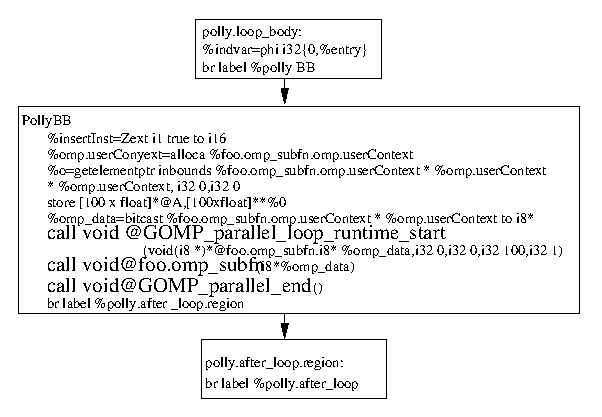
\includegraphics[width=1\textwidth]{images/ompcalls.eps}
  \caption{CFG showing sequence of OpenMP library calls}
\end{figure}

The control flow graph corresponding to the simple code in ~\ref{fig:openmp1} is shown in ~\ref{fig:openmp_cfg}
The code for body of the for loop is generated inside the subfunction which has the following GOMP library
calls to achieve the necessary parallelism.

\begin{itemize}
\item GOMP\_loop\_runtime\_next
\item GOMP\_loop\_end\_nowait
\end{itemize}

The signature and descriptions of each of the above functions can be found in in libgomp manual\cite{libgomp}.

\section{Support for inner loops}

So far OpenMP code created apply only for outermost loops, which is detected as SCoP. Next step is to do it for
inner loops. Due to dependency issues the outer loop is not detected as SCoP, but innerloop can be safely
parallelized as in the following example.

\begin{lstlisting}
  for (int i = 0; i < M; i++)
    for (int j = 0; j < N; j++)
      A[j] += M;
\end{lstlisting}

Those loops need the values of the surrounding induction variables and parameters in the OpenMP subfunction. We need
to pass the values of the outer induction variables in a structure to the subfunction. All the required variables
were already available in a datastructure used by Polly. We just needed to copy those into the body of the subfunction
so that it can refer those whenever needed.

\section{Adding OpenMP testcases}

<give more explanation>

\section{Dealing with memory references}

\begin{lstlisting}
#define N 10
  void foo() {
    float A[N];
    for (int i=0; i < N; i++)
      A[i] = 10;
    return;
}
\end{lstlisting}

Consider the above code segement. The 'for' loop will be detected as parallel by Polly and will be embedded in the
body of the OpenMP subfunction. But it accesses a non-global array 'A' and so accessing the same will not be possible inside
the subfunction. The approach for solving this issue is explained below.

\subsection{Adding memory references}

The base addresses of all memory references made by a statement is available in each statement instance. Prior to creating the body
of the subfunction we add all these base addresses are added into the same data structure where we stored the induction variables and parameters.
And then it is added to the subfunction structure.

\subsection{Extracting memory references}

Inside the body of the subfunction the base addresses are extracted from the subfunction structure and a new LLVM load instruction is created for each. The
new base addresses mapped to the old addresses so that any future references are made on the new addresses.



%%%%%%%%%%%%%%%%%%%%%%%%%%%%%%%%%%%%%%%%%%%%%%%%%%%%%%%%%%%%
% testing
\chapter{Testng with pollybench}
\label{chap:testing}
\section{PolyBench}
The framework is tested with polyBench 1.0\footnote{\url{http://www-roc.inria.fr/~pouchet/software/polybench/}} and the results are shown in the next section.
PolyBench is a set of computation intensive programs often used in the polyhedral community.
On those benchmarks Polly extracts the relevant SCoPs and optimizes them automatically.

\section{Experimental results}
\begin{figure}
\begin{center}
  %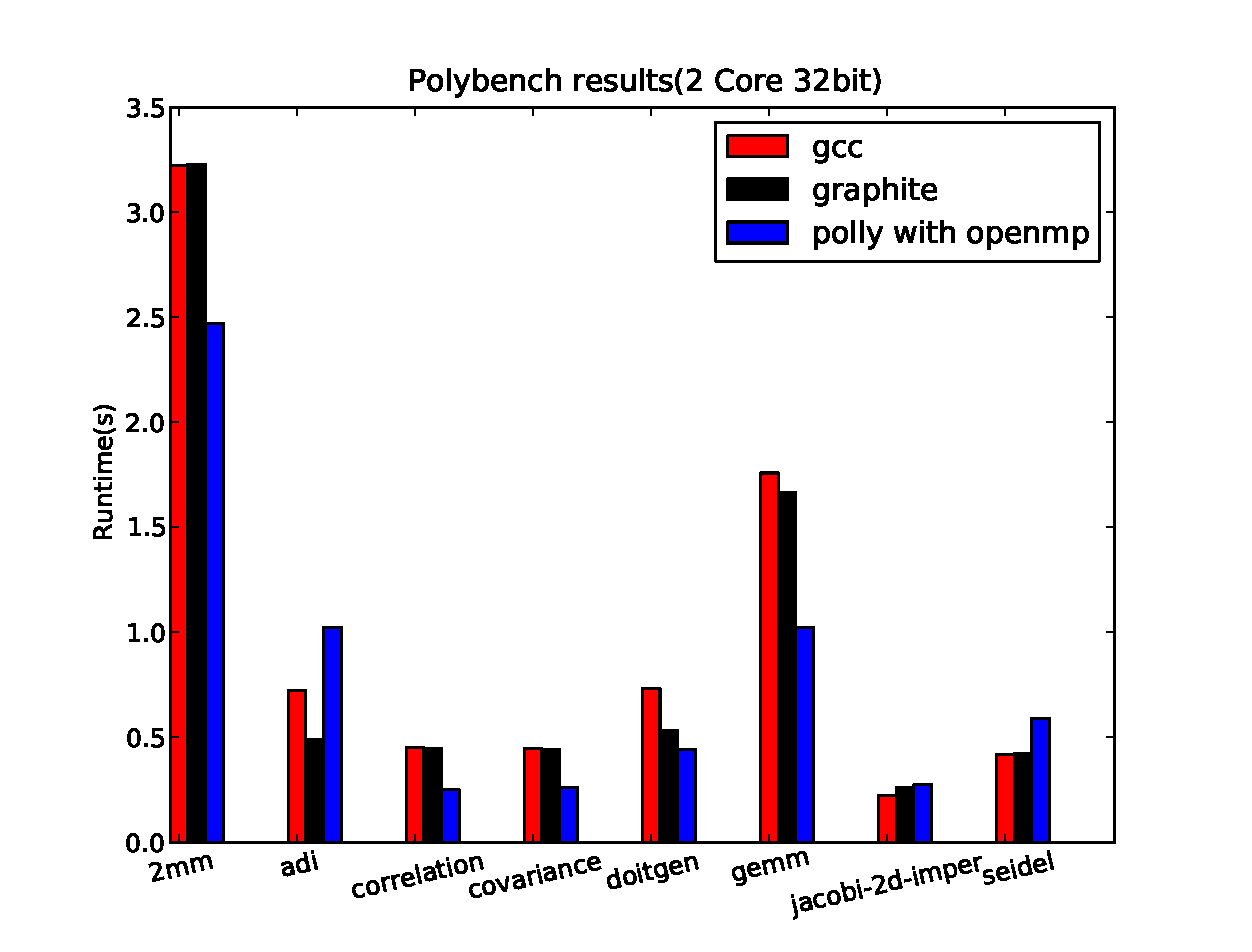
\includegraphics[width=1\textwidth]{images/2core32bit.eps}
  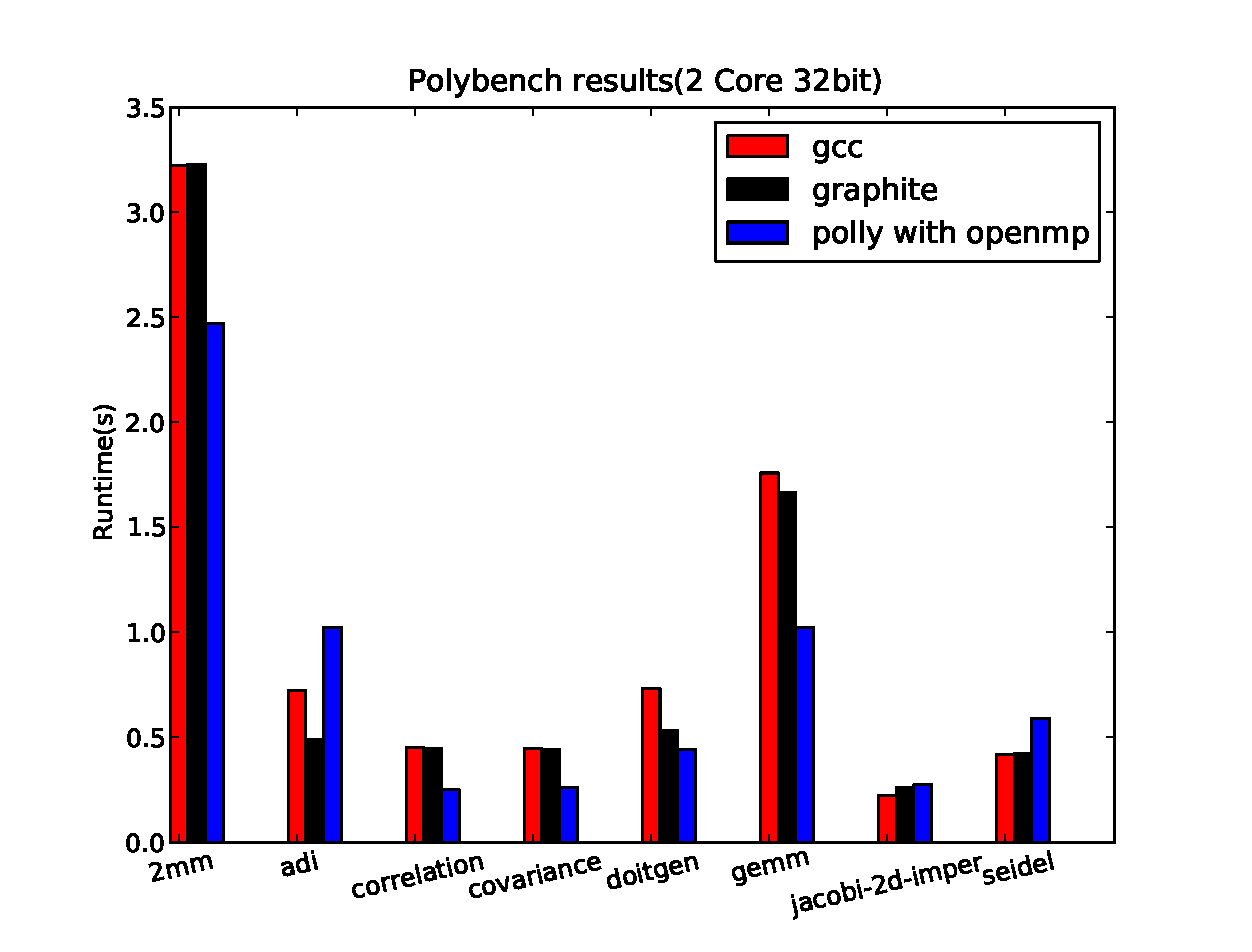
\includegraphics[height=9cm]{images/2core32bit.eps}
  \caption{Performance comparison(2 core 32 bit)}
  \label{fig:2core1}
\end{center}
\end{figure}

\begin{figure}
\begin{center}
  %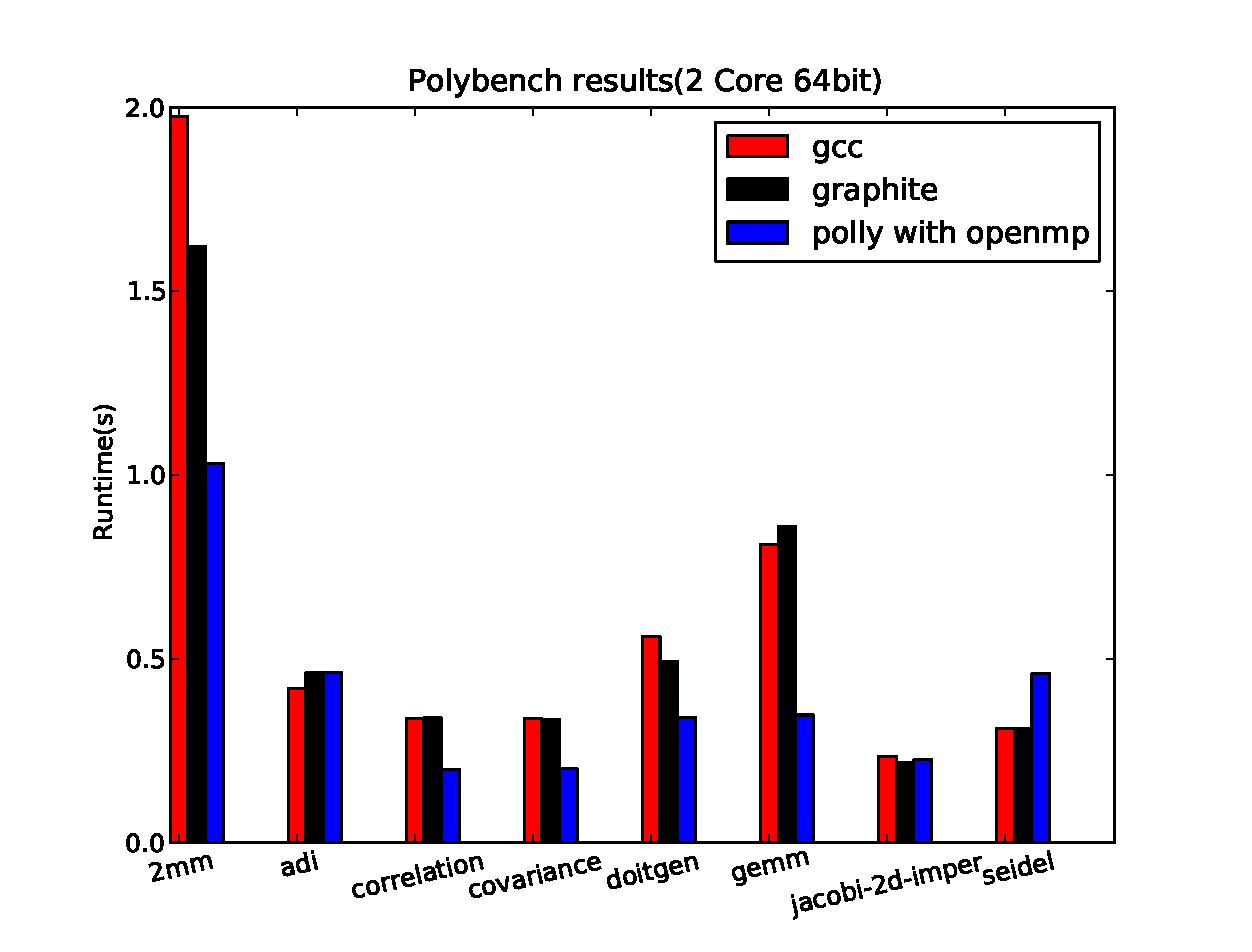
\includegraphics[width=1\textwidth]{images/2core64bit.eps}
  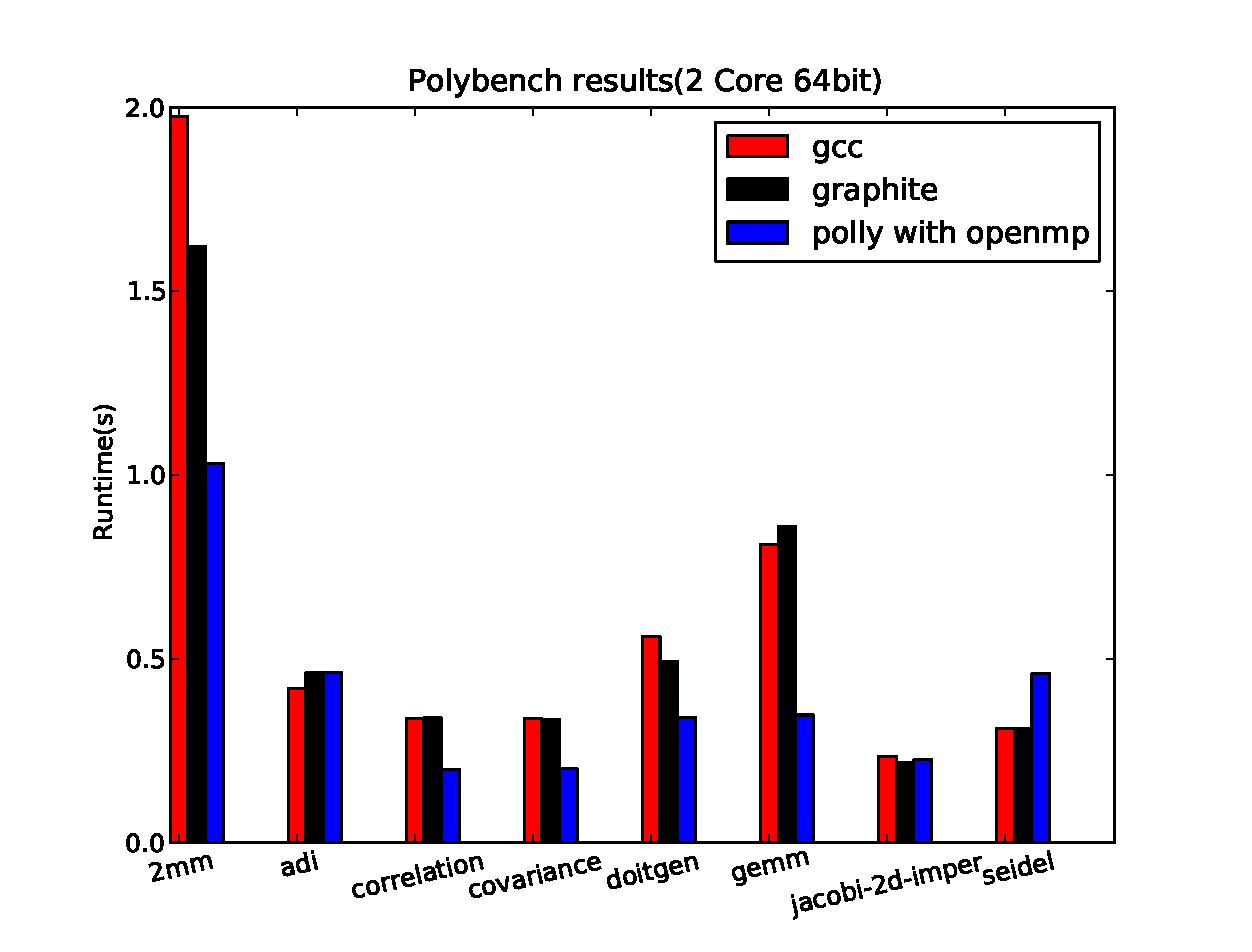
\includegraphics[height=9cm]{images/2core64bit.eps}
  \caption{Performance comparison(2 core 64bit)}
  \label{fig:2core2}
\end{center}
\end{figure}

\begin{figure}
\begin{center}
  %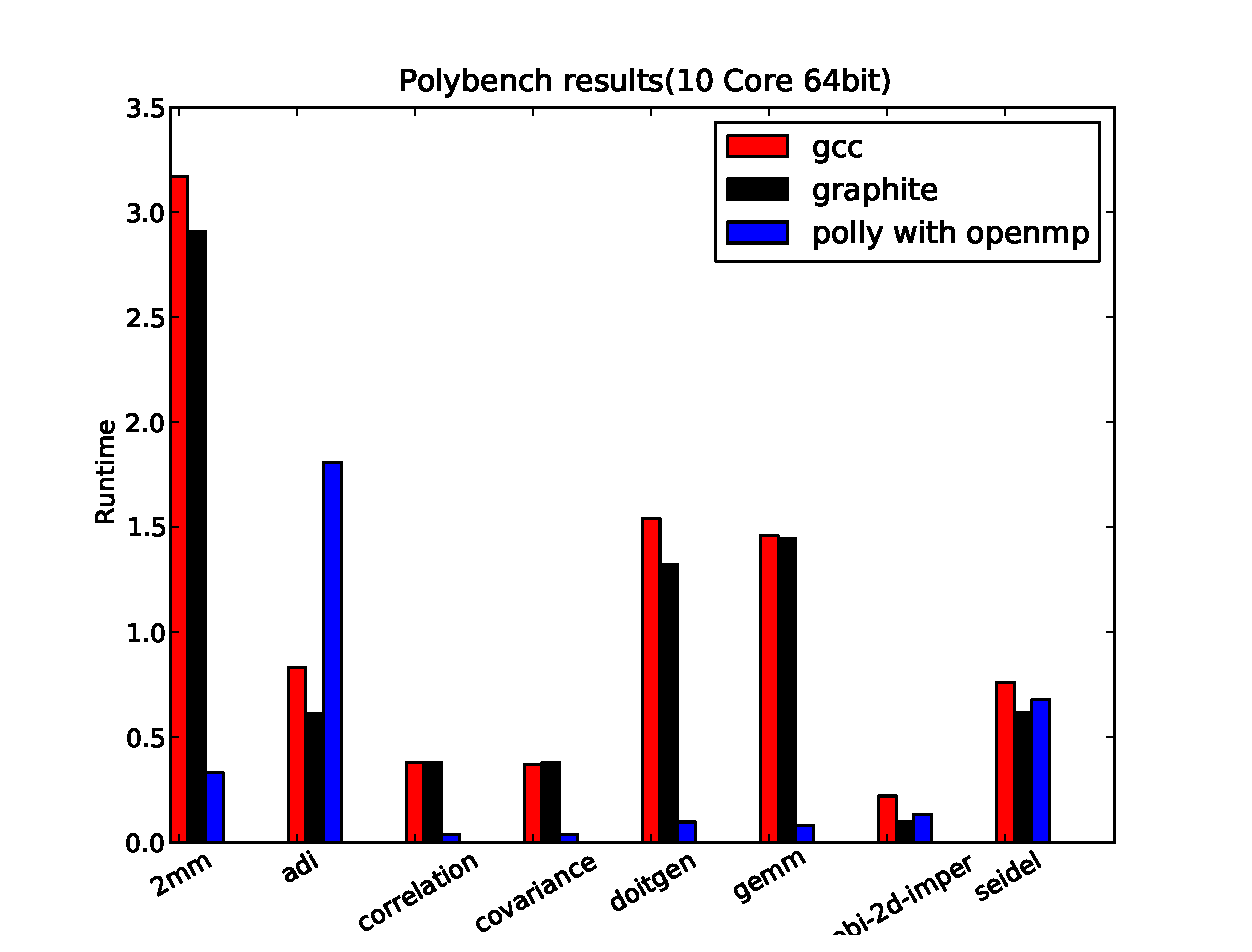
\includegraphics[width=1\textwidth]{images/10core64bit.eps}
  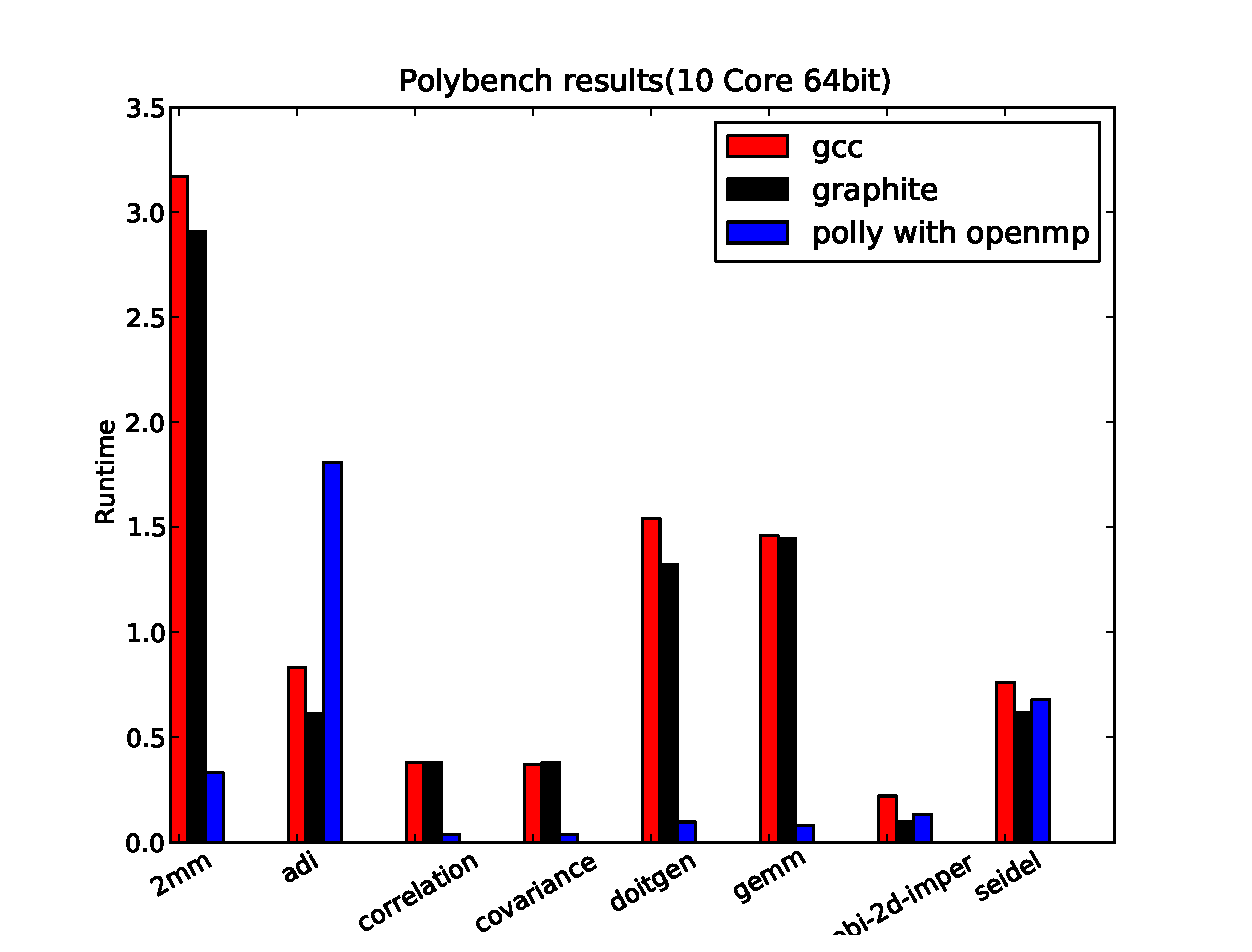
\includegraphics[height=9cm]{images/10core64bit.eps}
  \caption{Performance comparison(10 core 64 bit)}
  \label{fig:10core}
\end{center}
\end{figure}

The OpenMP code generated by Polly is compared with gcc and graphite\cite{TRIFUNOVIC:2010}. With gcc
we make a comparison with serial execution and with graphite we make comparison
with an existing autoparallelization framework, which is also based on polyhedral
model. 
The tests are carried out in 3 different machine with the following configuration

\begin{itemize}
\item Intel Core 2 Duo with 32 Bit OS
\item Intel Core 2 Duo with 64 bit OS
\item 10 Core AMD Engineering Sample with 64 Bit OS
\end{itemize}
The 10 core machine is part of GCC compile farm\footnote{\url{http://gcc.gnu.org/wiki/CompileFarm}}. The GCC Compile farm project maintains
a set of machines of various architectures and provides ssh access to free software developers, GCC and others.
Once the account application  is approved, we get full ssh access to all the farm machines. Then we
are free to install any packages and test our work. The only prerequisite to get access is that
we should be an active contributer for at least one free software project.

The script for testing is given below and the results are shown in the graphs in
Figures ~\ref{fig:2core1}, ~\ref{fig:2core2} and ~\ref{fig:10core}.
{\footnotesize
\begin{lstlisting}
# serial
gcc -I utilities utilities/instrument.c -DPOLYBENCH_TIME   \
                      -DPOLYBENCH_DUMP_ARRAYS -O3 $1 -lm
# Autopar with graphite
gcc -I utilities utilities/instrument.c -DPOLYBENCH_TIME   \
           -DPOLYBENCH_DUMP_ARRAYS -O3 -floop-interchange  \
           -floop-block -floop-parallelize-all             \
	   -ftree-parallelize-loops=2 $1 -lm
# Autopar with polly OpenMP
pollycc -fpolly -fparallel -I utilities utilities/instrument.c \
              -DPOLYBENCH_TIME -DPOLYBENCH_DUMP_ARRAYS  $1 -lm
\end{lstlisting}
}
While we look into the results it can be observed that Polly with OpenMP support
shows nice performance other than the benchmarks 'adi' and 'seidel'. It is observed
that the core loops in these testcases are detected as SCoPs and detected as parallel. OpenMP
code is generated for them too. The reason for the overhead is still to be investigated and such cases will be part of one
of the future works(Increasing coverage of Polly). For details refer to Chapter ~\ref{chap:future}.





%%%%%%%%%%%%%%%%%%%%%%%%%%%%%%%%%%%%%%%%%%%%%%%%%%%%%%%%%%%%
% gccvsllvm
%\chapter{Comparison of GCC and LLVM}
%

Forwarded conversation
Subject: [LLVMdev] LLVM vs GCC binary performance
------------------------

From: Yuli Fiterman <fiterman@gmail.com>
Date: Fri, Mar 11, 2011 at 12:44 PM
To: llvmdev@cs.uiuc.edu


Dear LLVM Team,

     As a developer I'm very excited and interested in the LLVM project. Though my knowledge of the details is cursory my general understanding is that the SSA code that LLVM front ends produce is supposed to allow for optimizations that are unfeasible in GCC. I also expect most important optimizations from GCC would have been incorporated into LLVM by now since GCC code is open for everyone to see. Therefore I'm surprised to see that in most benchmarks LLVM produces binaries are 10-15% slower than their GCC counterparts.  Would you mind explaining the main reasons for why this is the case? Also, what remains to be done for LLVM to surpass GCC in terms of binary performance?

     Thanks,
     Yuli
      

     _______________________________________________
     LLVM Developers mailing list
     LLVMdev@cs.uiuc.edu         http://llvm.cs.uiuc.edu
     http://lists.cs.uiuc.edu/mailman/listinfo/llvmdev


     ----------
     From: Duncan Sands <baldrick@free.fr>
     Date: Fri, Mar 11, 2011 at 8:23 PM
     To: llvmdev@cs.uiuc.edu


     Hi Yuli,
     not so, GCC also uses SSA form.  I'm not aware of any optimization that LLVM can
     do that GCC couldn't do if it tried.
     This is not the case.  You make it sound like reimplementing optimizations is
     a five minute job while that is very far from true!  Not to mention that GCC is
     a moving target: it is being worked on too and getting nice improvements all the
     time.  For example it has auto-vectorization support while LLVM does not.  Also,
     don't forget that LLVM is not simply GCC written in C++: it makes a lot of
     different design choices to GCC, and has a bunch of use cases that GCC does not,
     for example, the ability to JIT code.  The LLVM developers may feel that the way
     GCC solved some problem is not the best way for LLVM to solve it, and even if
     they think GCC's approach to some problem is great it nonetheless might be hard
     to do things the same in LLVM due to the different design.
     While in my experience this used to be pretty systematically true on x86
     linux, nowadays it is much more hit and miss: I see some programs running
     faster when compiled with LLVM, and others running faster when compiled with
     GCC.  On the whole I would say that on my machine GCC usually results in faster
     programs.
     On the whole GCC produces excellent code.  Many fine engineers have worked hard
     on it for many years, and it shows.  Doing better than GCC is difficult.
     There's no magic bullet.  The things to improve that would give you the most
     bang for your buck are probably the code generator and auto-vectorization.
     Increasing the number of developers would be helpful.

     Ciao, Duncan.
     _______________________________________________
     LLVM Developers mailing list
     LLVMdev@cs.uiuc.edu         http://llvm.cs.uiuc.edu
     http://lists.cs.uiuc.edu/mailman/listinfo/llvmdev

     ----------
     From: Renato Golin <rengolin@systemcall.org>
     Date: Fri, Mar 11, 2011 at 11:12 PM
     To: Duncan Sands <baldrick@free.fr>
     Cc: llvmdev@cs.uiuc.edu


     I'm not a GCC expert, but their auto-vectorization is not that great.
     It may be simple to do basic loop transformations and some stupid
     vectorization, but having a really good vectoriser is a lot of work.

     I personally think that the biggest difference is the number of people
     that have contributed over the years on very specific optimizations.
     There are as many corner cases as there are particles in the universe
     (maybe more), and implementing each one of them requires time and
     people willing. LLVM has the latter, but lacks the former, for now.

     Spending a full year on a vectoriser prototype might bring less value
     than the same year optimizing micro-benchmarks against GCC...

     Not that I don't think we should have a vectoriser, Poly is going to
     be great! But until it's not (and it's going to take some time), we
     better focus on some magic, as GCC did over the decades.

     My tuppence,

     --renato

     ----------
     From: Tobias Grosser <grosser@fim.uni-passau.de>
     Date: Sat, Mar 12, 2011 at 12:16 AM
     To: llvmdev@cs.uiuc.edu


     Hi,

     in case you are referring to PoLLy*, thanks for this nice comment. We
     can already do some basic vectorization and are currently working on
     increased coverage and enhanced robustness. I have already seen some
     nice speedups on some micro kernels, but need to get more confidence
     before I present them. I will also talk PoLLy on IMPACT/CGO 2011** , in
     case someone is around.
     Yes. Also for a vectorizer to be efficient you need to have a lot of
     magic and canonicalization done beforehand, to enable it to do a decent
     job. LLVM is actually pretty good in this respect.

     Cheers
     Tobi

     * Like Polly the parrot
     ** impact2011.inrialpes.fr

     ----------
     From: Renato Golin <rengolin@systemcall.org>
     Date: Sat, Mar 12, 2011 at 1:42 AM
     To: Tobias Grosser <grosser@fim.uni-passau.de>
     Cc: llvmdev@cs.uiuc.edu


     Hi Tobias,

     This is not the first time you correct me, sorry, but yes, I was
     talking about PoLLy. ;)

     cheers,
     --renato




     -- 
     Raghesh
     II MTECH
     Room No: 0xFF
     Mahanadhi Hostel
     IIT Madras
     


%%%%%%%%%%%%%%%%%%%%%%%%%%%%%%%%%%%%%%%%%%%%%%%%%%%%%%%%%%%%


% Appendices.

\appendix
 
\chapter{Various Tools used in Polyhedral community}
\section{Isl}
\section{Polylib}
\section{Cloog}
\section{PluTo}
\section{Piplib}

\chapter{Doing Projects - The Open Source Way}
 
 Just put in text as you would into any chapter with sections and
 whatnot.  Thats the end of it.

%%%%%%%%%%%%%%%%%%%%%%%%%%%%%%%%%%%%%%%%%%%%%%%%%%%%%%%%%%%%
% List of papers

\chapter*{Publications}
\vspace{-0.3cm}

\begin{enumerate}
\item Tobias Grosser, Hongbin Zheng, Raghesh Aloor, Andreas Simb{\"u}rger, Armin {G}r{\"o}{\ss}linger and Louis-No{\"e}l Pouchet \newblock
  Polly - Polyhedral optimization in LLVM \newblock {\em
  IMPACT 2011(First International workshop on PolyhedrAl Compilation Techniques)}, Chamonix, France.
\end{enumerate}

%\nocite{bellman, Amarel:1968, manning, knoblock90learning,
%crawford92theoretical, Barto:rtdp, Ravindran:proof}

%%%%%%%%%%%%%%%%%%%%%%%%%%%%%%%%%%%%%%%%%%%%%%%%%%%%%%%%%%%%
% Bibliography.
\pagebreak
\begin{singlespace}
  \begin{small}
	\bibliography{refs}
%\bibliographystyle{plain}
  \end{small}
\end{singlespace}

%%%%%%%%%%%%%%%%%%%%%%%%%%%%%%%%%%%%%%%%%%%%%%%%%%%%%%%%%%%%

\end{document}
